% A LaTeX template fitted for a Phd thesis report
% Copyright (C) 2013 Damien Roque
% Author : Damien Roque <damien.roque_AT_isae-supaero.fr>

\documentclass[a4paper,12pt,twoside]{templates/roque-phdthesis-template}

% Include configuration (loading packages, defining the style of the document...)
\usepackage[utf8]{inputenc}
% Encoding and internationalization
\usepackage[T1]{fontenc}
\usepackage{aecompl}
%\usepackage{natbib}
\usepackage[french]{babel} % Comment this line if the document is written in english
%\usepackage[american]{babel} % Comment this line if the document is written in english
\usepackage{csquotes}


% Title page from the University of Toulouse (see doc for further explanations)
\usepackage[ED=MITT-STICRT, Ets=ISAE]{templates/tlsflyleaf}

\title{Le titre de la thèse}
\author{Prénom NOM}
\defencedate{Date de défense (JJ/MM/AAAA)}
\lab{Nom du laboratoire (UMR)}
%\cotutelle{Institut de cotutelle}

%% Directeur(s) de thèse
\nboss{2}                                    % Nombre de directeur(s) de thèse
\makesomeone{boss}{2}{Second DIRECTEUR}{}{}  % Sera affiché en second
\makesomeone{boss}{1}{Premier DIRECTEUR}{}{} % Sera affiché en premier
%% Referee
\nreferee{2}
\makesomeone{referee}{1}{Premier RAPPORTEUR}{}{}
\makesomeone{referee}{2}{Second RAPPORTEUR}{}{}
%% Jury
\njudge{3}
\makesomeone{judge}{1}{Premier MEMBRE}{Professeur d'Université}{Président du Jury}
\makesomeone{judge}{2}{Second MEMBRE}{Astronome Adjoint}{Membre du Jury}
\makesomeone{judge}{3}{Troisième MEMBRE}{Chargé de Recherche}{Membre du Jury}

% Math packages
\usepackage{amsmath,amssymb}
\usepackage{mathrsfs}
\usepackage{amsthm}
\usepackage{a4wide}
\renewcommand{\baselinestretch}{1.05}

% Graphics and hyperlinks
\usepackage[hyperindex=true]{hyperref}
\usepackage{url}
\usepackage{hyperref}
\graphicspath{{.}{images/}}
\usepackage{eso-pic}
\usepackage{rotating}
%\usepackage[font=normalsize]{subfig}
\usepackage{tikz}
\usetikzlibrary{shapes,arrows}
\usepackage{pgfplots}
\pgfplotsset{compat=newest}
\pgfplotsset{plot coordinates/math parser=false}
\newlength\figureheight
\newlength\figurewidth
\usepackage{caption}
\usepackage{subcaption}
\usepackage{subfig}
\usepackage{subfigure}

\pgfkeys{/pgf/number format/.cd,
set decimal separator={,\!},
1000 sep={\,},
} % Comment this line if the document is written in english

\usetikzlibrary{plotmarks}
\usepackage{pdfpages}

\usepackage[strict]{changepage}
\newcommand\BackgroundPic{
\put(0,0){
\parbox[b][\paperheight]{\paperwidth}{%
\vfill
\centering
\includegraphics[width=0.9\paperwidth,height=1\paperheight,keepaspectratio]{images/background-eps-converted-to}%
\vfill
}}}

\usepackage{color}
\definecolor{linkcol}{rgb}{0,0,0} 
\definecolor{citecol}{rgb}{0,0,0}

\hypersetup
{
bookmarksopen=true,
pdftitle={Mon sujet de thèse complet},
pdfauthor={Prénom NOM},
pdfsubject={Rapport de thèse},
pdfmenubar=true,
pdfhighlight=/O,
colorlinks=true,
pdfpagelayout=SinglePage,
pdffitwindow=true,
linkcolor=linkcol,
citecolor=citecol,
urlcolor=linkcol
}



% Headers and footers
\usepackage{fancyhdr}
\fancyhf{}
\rhead{2018/2019}
\lhead{\nouppercase{\leftmark}}
\pagestyle{fancy}
\fancyfoot{}
%\fancyhead[LE,RO]{\bfseries\thepage}
%\fancyhead[RE]{\bfseries\nouppercase{\leftmark}}
%\lyhead{\leftmark}

\let\headruleORIG\headrule
\renewcommand{\headrule}{\color{black} \headruleORIG}
\renewcommand{\headrulewidth}{1.0pt}
\usepackage{colortbl}
\arrayrulecolor{black}

%\fancypagestyle{plain}{
 % \fancyhead{}
 \fancyfoot[C]{\thepage}
 % \renewcommand{\headrulewidth}{0pt}
%}

\usepackage[footnote]{acronym}

% Mini table of content and acronyms
\usepackage[nottoc, notlof, notlot]{tocbibind}
%\usepackage{natbib}
\usepackage[french]{minitoc}
\setcounter{minitocdepth}{3}
\mtcindent=15pt
\setlength{\parskip}{10pt}

\let\minitocORIG\minitoc
\renewcommand{\minitoc}{\minitocORIG \vspace{1.5em}}

\setcounter{secnumdepth}{3}
\setcounter{tocdepth}{3}
\usepackage{silence}

\WarningFilter{minitoc(hints)}{W0023}
\WarningFilter{minitoc(hints)}{W0024}
\WarningFilter{minitoc(hints)}{W0028}
\WarningFilter{minitoc(hints)}{W0030}

% References formatting
% Bibtex
% \renewcommand*{\backref}[1]{}
% \renewcommand*{\backrefalt}[4]{%
% \ifcase #1 %
% (Non cité.)%
% \or
% (Cité en page~#2.)%
% \else
% (Cité en pages~#2.)%
% \fi}
% \renewcommand*{\backrefsep}{, }
% \renewcommand*{\backreftwosep}{ et~}
% \renewcommand*{\backreflastsep}{ et~}
\usepackage{natbib}
% BibLatex
\usepackage[style=numeric,backend=bibtex,isbn=false,doi=false,backref=true,url=false]{biblatex}
\addbibresource{references.bib}
\inputencoding{utf8}

% Pages succession
\makeatletter
\def\cleardoublepage{\clearpage\if@twoside \ifodd\c@page\else%
  \hbox{}%
  \thispagestyle{empty}%
  \newpage%
  \if@twocolumn\hbox{}\newpage\fi\fi\fi}
\makeatother

\newenvironment{vcenterpage}
{\newpage\vspace*{\fill}\thispagestyle{empty}\renewcommand{\headrulewidth}{0pt}}
{\vspace*{\fill}}

%%% Local Variables: 
%%% mode: latex
%%% TeX-master: "../phdthesis"
%%% End: 


% Include user's macros
% Math macros
\newcommand*{\SET}[1]  {\ensuremath{\mathrm{\mathbf{#1}}}}
\newcommand*{\VEC}[1]  {\ensuremath{\boldsymbol{#1}}}
\newcommand*{\MAT}[1]  {\ensuremath{\boldsymbol{#1}}}
\newcommand*{\OP}[1]  {\ensuremath{\boldsymbol{\mathcal{#1}}}}
\newcommand*{\ESP}[1]  {\ensuremath{ \mathbb{E} \left \{#1 \right \}}}
\newcommand*{\ESPENS}[2]  {\ensuremath{ \mathbb{E}_{#1} \left \{#2 \right \}}}
\newcommand*{\NORM}[1]  {\ensuremath{\left\|#1\right\|}}
\newcommand*{\DPR}[2]  {\ensuremath{\left \langle #1,#2 \right \rangle}}
\newcommand*{\FOURIER}[1]  {\ensuremath{\widehat{#1}}}
\newcommand{\eqdef}{\stackrel{\mathrm{def}}{=}}
\newcommand{\argmax}{\operatornamewithlimits{argmax}}
\newcommand{\argmin}{\operatornamewithlimits{argmin}}
\newcommand{\diag}{\operatorname{diag}}
\newcommand{\ud}{\, \mathrm{d}}
\newcommand{\vect}{\mathrm{Vect}}
\newcommand{\sinc}{\mathrm{sinc}}
\newcommand{\esp}{\ensuremath{\mathrm{E}}} % Problème pour les short captions
\newcommand{\hilbert}{\ensuremath{\mathcal{H}}}
\newcommand{\supps}{\ensuremath{\tilde{\mathrm{supp}}}}
\newcommand{\supp}{\ensuremath{\mathrm{supp}}}
\newcommand{\sgn}{\mathrm{sgn}}
\newcommand{\intTT}{\int_{-T}^{T}}
\newcommand{\intT}{\int_{-\frac{T}{2}}^{\frac{T}{2}}}
\newcommand{\intinf}{\int_{-\infty}^{+\infty}}
\newcommand{\iintinf}{\iint_{-\infty}^{+\infty}}
\newcommand{\iintrr}{\iint\limits_{\SET{R}^2}}
\newcommand{\intr}{\int\limits_{\R}}
\newcommand{\Sh}{\ensuremath{\boldsymbol{U}}}
\newcommand{\C}{\ensuremath{\mathbf{C}}}
\newcommand{\R}{\ensuremath{\mathbf{R}}}
\newcommand{\Z}{\ensuremath{\mathbf{Z}}}
\newcommand{\N}{\ensuremath{\mathbf{N}}}
\newcommand{\K}{\ensuremath{\mathbf{K}}}
\newcommand{\reel}{\mathcal{R}}
\newcommand{\imag}{\mathcal{I}}
\newcommand{\cmnr}{c_{m,n}^\reel}
\newcommand{\cmni}{c_{m,n}^\imag}
\newcommand{\cnr}{c_{n}^\reel}
\newcommand{\cni}{c_{n}^\imag}
\newcommand{\tproto}{g}
\newcommand{\rproto}{\check{g}}
\newcommand{\Tproto}{G}
\newcommand{\Rproto}{\check{G}}
\newcommand{\Tpoly}{F}
\newcommand{\Rpoly}{\check{F}}
\newcommand{\estim}{\tilde{c}}
\newcommand{\egal}{\bar{c}}
\newcommand{\bb}{b}
\newcommand{\bbf}{z}
\newcommand{\bbr}{\zeta}
\newcommand{\LR}{\mathcal{L}_2(\R)}
\newcommand{\LRR}{\mathcal{L}_2(\R^2)}
\newcommand{\LZ}{\ell_2(\Z)}
\newcommand{\LZZ}{\ell_2(\Z^2)}
\newcommand{\peigne}{\ensuremath{\Psi}}
\newcommand{\avec}{\qquad \text{avec} \qquad}

% Theorems definition
\newtheoremstyle{break}
  {11pt}{11pt}%
  {\itshape}{}%
  {\bfseries}{}%
  {\newline}{}%
\theoremstyle{break}

\newtheorem{definition}{Définition}[chapter]
\newtheorem{theoreme}{Théorème}[chapter]
\newtheorem{remarque}{Remarque}[chapter]
\newtheorem{propriete}{Propriété}[chapter]
\newtheorem{exemple}{Exemple}[chapter]

% Example of background tag
% \AddToShipoutPicture{%
% \begin{tikzpicture}[remember picture,overlay]
%   \node [rotate=60,scale=10,text opacity=0.1] at (current page.center) {Brouillon};
% \end{tikzpicture}}

% Example of header tag
% \AddToShipoutPicture{%
% \tikzstyle{block} = [draw, thick, color=blue, scale=1.5,rectangle, minimum height=3em, minimum width=6em]
% \begin{tikzpicture}[remember picture,overlay]
%   \node [coordinate] at (current page.north) (accroche) {};
%   \node [block, below of=accroche] {Diffusion restreinte};
% \end{tikzpicture}}

% Another example of header tag
% \AddToShipoutPicture{%
% \tikzstyle{block} = [draw, thick, color=red, scale=1.5,rectangle, minimum height=3em, minimum width=6em]
% \begin{tikzpicture}[remember picture,overlay]
%   \node [coordinate] at (current page.north) (accroche) {};
%   \node [block, below of=accroche] {Confidentiel Défense};
% \end{tikzpicture}}

%%% Local Variables: 
%%% mode: latex
%%% TeX-master: "../phdthesis"
%%% End: 

% Build only the following parts of the document (recommended for large documents)
% \chapter*{Introduction Générale}
\addstarredchapter{Introduction Générale}
\markboth{Introduction}{Introduction}
\label{chap:introduction}
%\minitoc

Le développement technologique rapide a permis aux véhicules de devenir l’un des moyens de transport les plus confortables et fiables. Cependant, des phénomènes alarmants lies à la circulation routière sont apparus tels que la congestion bloquante et les accidents mortels. Chaque année, environ 40.000 personnes meurent sur les routes, et 1,7 millions autres sont grièvement blessées \cite{25}. Autre que les dégâts humains, les coûts annuels engendrés par les accidents de la route s’élèvent à près de 3 \% du PIB mondial, et le problème continue à s’aggraver à cause de la disparité entre le rythme de construction de routes et le nombre de véhicules qui les occupent chaque année. \\

D'autre part, les panneaux de signalisation routière constituent un élément important dans l’organisation et la sécurisation du trafic routier. Leurs respect réduit considérablement le nombre et l’impact des accidents. De nos jours, la disponibilité du matériel et du logiciel performants, ainsi que l’avancement notable dans le domaine d’apprentissage automatique ont rendu possible le développement de systèmes robustes pour la détection et de reconnaissance automatique de panneaux de signalisation routière.  De tels systèmes permettront, par exemple, d’alerter le conducteur de la présence d’un signe de « Stop », de « Sens interdit » dont l’inattention du conducteur peut découler à un dégât mortel. Ce même système est indispensable pour les véhicules autonomes qui sont déjà sur les routes des payes développés. D’autant plus, la reconnaissance automatique des plaques aide dans l’entretien des panneaux défectueux qui est une tache fastidieuse qui doit se faire périodiquement. Pour ces raisons, de tels systèmes attirent de plus en plus l’attention des industriels de l’automobile. Certains modèles de véhicules haut de gamme sont déjà équipés de fonctionnalité de détection automatique des panneaux sans qu’ils soient autonomes. \\

Dans la lumière de cette thématique, nous proposons une étude des algorithmes de reconnaissance des panneaux routiers en utilisant des techniques d’apprentissage profonds ou «\textit{Deep Leanring}». Plus particulièrement, nous nous intéressons aux architectures de réseaux de neurones profonds de type convolutif ou CNN (\textit{Convolutional Neural Networks}) – qui sont mieux adaptés aux taches de classification d’images. Plusieurs variantes de ces modèles seront comparées afin d’établir des choix fondés avant de développer une solution déployable. En plus, nous avons proposé une approche basée sur l’apprentissage a partir de données synthétiques pour remédier aux problèmes de différence d'apparence des signes à travers les pays et a l’insuffisance ou le déséquilibre de la quantité de données d’apprentissage.\\
 
Afin de mieux présenter les techniques étudiées et les résultats obtenus suite au travail effectué, le reste de ce mémoire est organisé en trois parties. Dans la première, nous présentons des généralités sur les panneaux de signalisation routière et leurs normalisations. Nous enchaînons avec des applications du système de reconnaissance automatique et quelques difficultés qui les entravent.

Dans la deuxième partie, divisée en deux chapitres, nous évoquons la détection ainsi que la reconnaissance des panneaux routiers. Nous présentons, d'abord,  l'état de l’art du domaine et les notions relatives a ces deux taches, puis une étude comparative entre les différentes méthodes de reconnaissance est effectuée. 

Nous entamons la troisième partie par un aperçu sur le \emph{Deep Learning} et nous mettons l’accent sur les CNN pour la classification des images. Une étude expérimentale approfondie sera par la suite menée pour montrer les performances de certaines variantes de CNN, en l'occurrence, le  \textbf{VGGnet 16} \cite{simonyan2014very} et \textbf{Inception} \cite{43022} sur les données de panneaux de signalisation routière \textbf{GTRSB} (German Traffic Sign Recognition Benchmark \cite{Stallkamp2012}), sur lesquelles nous avons effectué une étude comparative de leurs performance. Ensuite, et afin de résoudre le problème de quantité de données d'apprentissage nécessaires, nous étudions l'apport de données synthétiques, qui sont  plus faciles à obtenir et a manipuler.\\ 

Nous clôturons ce mémoire par une conclusion générale ou nous résumons les travaux que nous avons effectues et nous citerons quelques perspectives dans l'objectif de l’améliorer et d'orienter futurs travaux sur la même problématique.





 

%%% Local Variables: 
%%% mode: latex
%%% TeX-master: "../phdthesis"
%%% End: 

% \part{Concepts Fondamentaux }
\chapter{Reconnaissance des panneaux de signalisation routière}
\label{chap:premierchapitre}
\minitoc

Dans ce chapitre, nous allons voir des généralités sur les panneaux de signalisation routière ainsi que différentes applications des systèmes de détection et de reconnaissance automatiques tout en entamant les étapes principales du processus de la reconnaissance.

\section{Panneaux de signalisation routière}

Les panneaux de signalisation routière constituent un élément important de la circulation routière. Leur fonction principale est d’exposer et d’afficher le contenu qui doit avertir les conducteur des dangers potentiels ainsi que les informations sur la route. C’est pour cette raison que la détection et l’identification des panneaux de signalisation est un aspect de recherche très important dans la prévention des accidents au niveau de route (Figure- \ref{fig: panneaux-al}).

\begin{figure}[htp!]
     \centering
      \begin{subfigure}
          \centering    
              
\includegraphics[width=3.5cm,height=4cm]{images/ii.jpg}
              \end{subfigure}
           \hfill
     \begin{subfigure}
              \centering  
       
\includegraphics[width=3.5cm,height=4cm]{images/300.jpg}
     \end{subfigure}
          \hfill
     \begin{subfigure}
             \centering     
            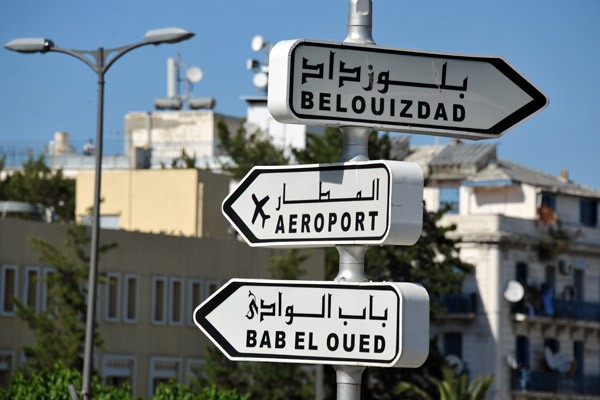
\includegraphics[width=3.5cm,height=4cm]{images/3.jpg}
     \end{subfigure}
           \hfill
     \begin{subfigure}
              \centering    
            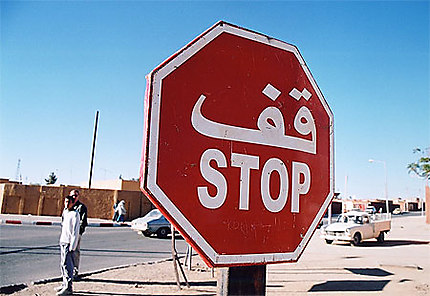
\includegraphics[width=3.5cm,height=4cm]{images/5.jpg}
     \end{subfigure}
      \caption{Exemples de plaques routières en Algérie}
       \label{fig: panneaux-al}
\end{figure}

\subsection{Classification des panneaux de signalisation routière }

Une convention sur la signalisation routière a été faite à Vienne le 8 novembre 1968. Cette dernière consiste en un  traité international qui a réuni un ensemble de pays (Figure- \ref{fig:participants de Viennes}), reconnaissant que l’uniformité et la normalisation des panneaux de signalisation, des feux de circulation de routes et des marquages, sont nécessaires pour gérer la circulation routière. \cite{1}.\\

\begin{figure}[h!]
        \centering
        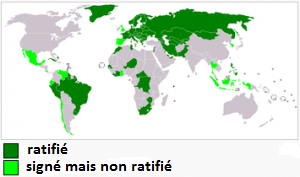
\includegraphics[width=8cm,height=4cm]{images/vienna.png}
        \caption{Participants à l’union de Vienne}
        \label{fig:participants de Viennes}
\end{figure}
    
A partir de cette réunion, plusieurs  articles ont été fournis parmi lesquelles l’article numéro "02" qui classe les panneaux de signalisation routière en catégories nommées de ‘A’  à ‘H’ contenant chacune un groupe de panneaux spécifiques (Tableau-\ref{table:classes de panneaux}).\\
Les sections principales issues de l’article sont:
\begin{table}[]
\centering
\begin{tabular}{|l|l|l|}
\hline
\multicolumn{1}{|c|}{code de la section} & \multicolumn{1}{|c|}{contenu} & \multicolumn{1}{|c|}{exemple}  \\ \hline
  \multicolumn{1}{|c|}{A }
  & 
  \multicolumn{1}{|c|}{Les panneaux d'avertissement de danger} 
  & 
 \multicolumn{1}{|c|}{
\includegraphics[width=2.5cm,height=2cm]{100.jpg}}   \\ \hline
  \multicolumn{1}{|c|}{B}    &
\multicolumn{1}{|c|}{Les signes de priorité} 
& \multicolumn{1}{|c|}{
\includegraphics[width=2.5cm,height=2cm]{101.jpg}} \\ \hline
 \multicolumn{1}{|c|}  {C}  
    & 
 \multicolumn{1}{|c|}   {Les signes d'interdiction ou de restriction}   & 
 \multicolumn{1}{|c|}  {
\includegraphics[width=2.5cm,height=2cm]{102.jpg} }\\ \hline
     \multicolumn{1}{|c|} {D} 
    & 
    \multicolumn{1}{|c|}{Les signes obligatoires}
    & 
     \multicolumn{1}{|c|} {
\includegraphics[width=2.5cm,height=2cm]{103.png}}  \\ \hline
      \multicolumn{1}{|c|}{E}  
    & 
    \multicolumn{1}{|c|}{Signalisation réglementaire spéciale}  
    & 
 \multicolumn{1}{|c|} {
\includegraphics[width=2.5cm,height=2cm]{sss.png}} \\  \hline  
  \multicolumn{1}{|c|} {F}   
    & 
    \multicolumn{1}{|c|}{Informations, installations ou panneaux de service} 
    & 
    \multicolumn{1}{|c|}{
\includegraphics[width=2.5cm,height=2cm]{exit.png}} \\      \hline 
   \multicolumn{1}{|c|}{G}
    & 
   \multicolumn{1}{|c|} {Panneau de direction, de position ou d'indication}
    & 
   \multicolumn{1}{|c|}{
\includegraphics[width=2.5cm,height=2cm]{104.jpg}} \\       \hline   
   \multicolumn{1}{|c|}{H } 
    & 
    \multicolumn{1}{|c|}{Panneaux supplémentaires} 
    & 
    \multicolumn{1}{|c|}{
\includegraphics[width=2.5cm,height=2cm]{images/200.png}} \\  \hline   
         
\end{tabular}
\caption{Classes de panneaux de signalisation routière}
\label{table:classes de panneaux}
\end{table}
\newpage
La convention, dans une deuxième partie, définit les couleurs, des tailles et des formes précises pour chacune de ces classes de signes.\\
Malgré les normalisations et les standards qui furent révisés plusieurs fois, il existe toujours des différences entre les pays contractés dans l’accord. Le tableau (Table-\ref{table:diff-p}) montre des panneaux indiquant la présence d'un passage piéton dans différents pays.\\
\begin{table}[]
\centering
\begin{tabular}{|l|l|l|}
\hline
\multicolumn{1}{|c|}{
\includegraphics[width=3cm,height=2.5cm]{images/pieton5.png}} & \multicolumn{1}{c|}{
\includegraphics[width=3cm,height=2.5cm]{images/pieton3.png}} & \multicolumn{1}{c|}{
\includegraphics[width=3cm,height=2.5cm]{images/pieton3.png}} \\ \hline
\multicolumn{1}{|c|}{En Malaisie}    & \multicolumn{1}{c|}{Au Japon }  & \multicolumn{1}{c|}{Aux Philippines}\\ \hline
\end{tabular}
\caption{Exemple de différence entre les panneaux de         signalisation routière}
\label{table:diff-p}
\end{table}
\subsection{Propriétés des panneaux de signalisations routière}

Les panneaux de signalisation ont été conçus pour être distincts des arrières plans naturels ou artificiels et ils ont des caractéristiques qui les rendent reconnaissables dans l’environnement. En général, ils sont fabriqués et installés conformément à des règles strictes (Figure- \ref{fig:formes}).
Les symboles sur les panneaux ont une couleur qui les distingue de l'arrière plan de la scène. La teinte de la peinture qui recouvre le signe correspond à une longueur d'onde spécifique dans le spectre visible. Les panneaux sont situés à des emplacements bien définis sur la route, de sorte que le conducteur peut s’attendre à les observer. Ils  peuvent contenir des pictogrammes, du texte ou les deux au même temps tout en prenant une forme géométrique particulière (cercle,triangle, rectangle, etc.)
\begin{figure}[h]
  \centering
  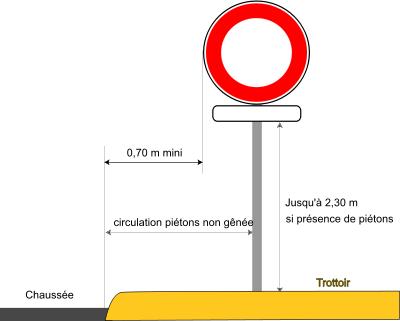
\includegraphics[width=7cm,height=5cm]{images/rte.png}
  \caption{Exemple de différentes règles d'implantations d'un panneau routier}
  \label{fig:formes}
\end{figure}

\newpage
\section{Domaines d’application}

La détection et la reconnaissance des panneaux de signalisation routière a prouvée un grand intérêt au cours des dernières années,cela est dû au large éventail d'applications qu'un système doté de cette capacité offre;

\subsection{Entretien des autoroutes}

Quotidiennement, un opérateur humain doit  vérifier la présence et l'état des panneaux au niveau des autoroutes (Figure-\ref{fig:entretien}).\\

\begin{figure}[h]
        \centering
        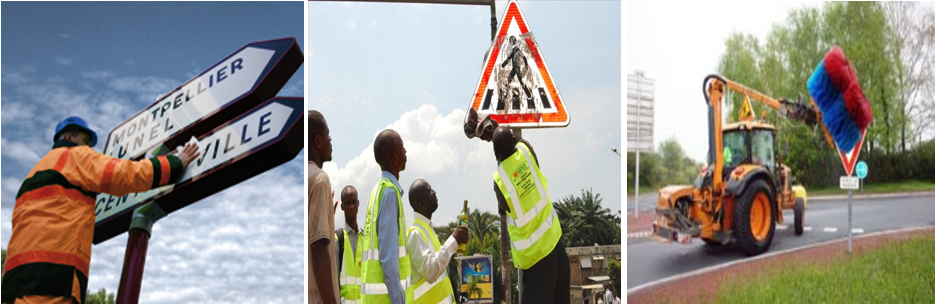
\includegraphics[width=10cm,height=3cm]{images/ccc.png}
        \caption{Entretien de panneaux routiers}
        \label{fig:entretien}
\end{figure}

C'est une tâche fastidieuse car les panneaux sont nombreux. Il y a un projet européen appelé "AUTOCAT" \cite{2} qui présente une fourgonnette développée pour la collecte automatique de la position et l'orientation des panneaux de signalisation routière (Figure- \ref{fig:vehicules de}) ci-dessus montre des véhicules modernes dans le même contexte.

\begin{figure}[h]
        \centering
        \begin{subfigure}
        \centering
        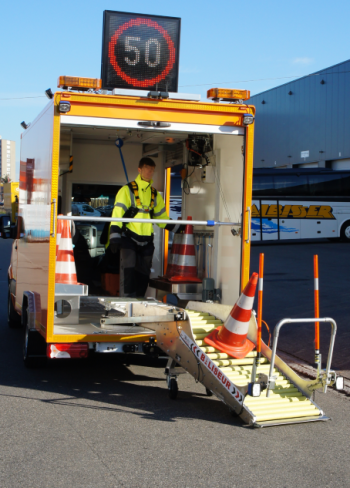
\includegraphics[width=4cm,height=4cm]{images/c1.png}  \end{subfigure}
         \begin{subfigure}
         \centering
        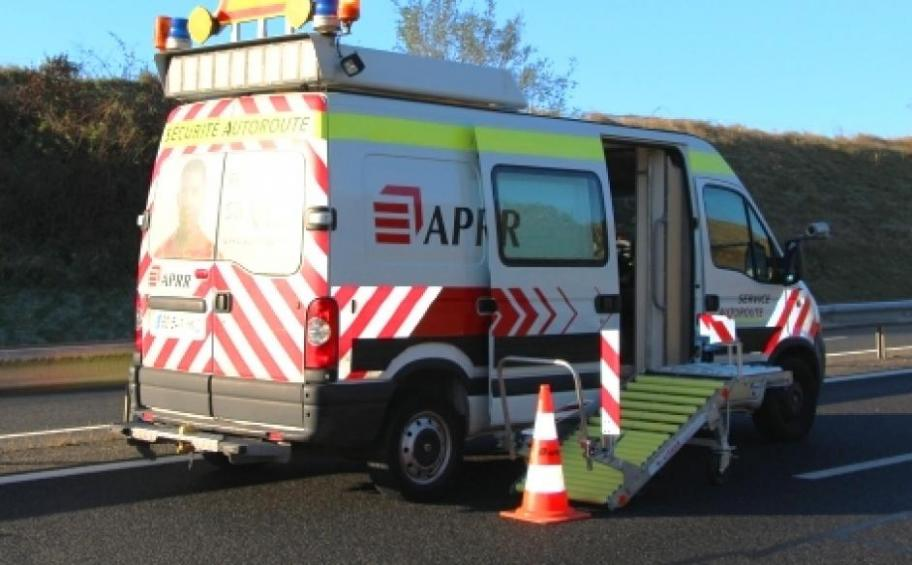
\includegraphics[width=4cm,height=4cm]{images/c2.png}
        \end{subfigure}
        \begin{subfigure}
        \centering
        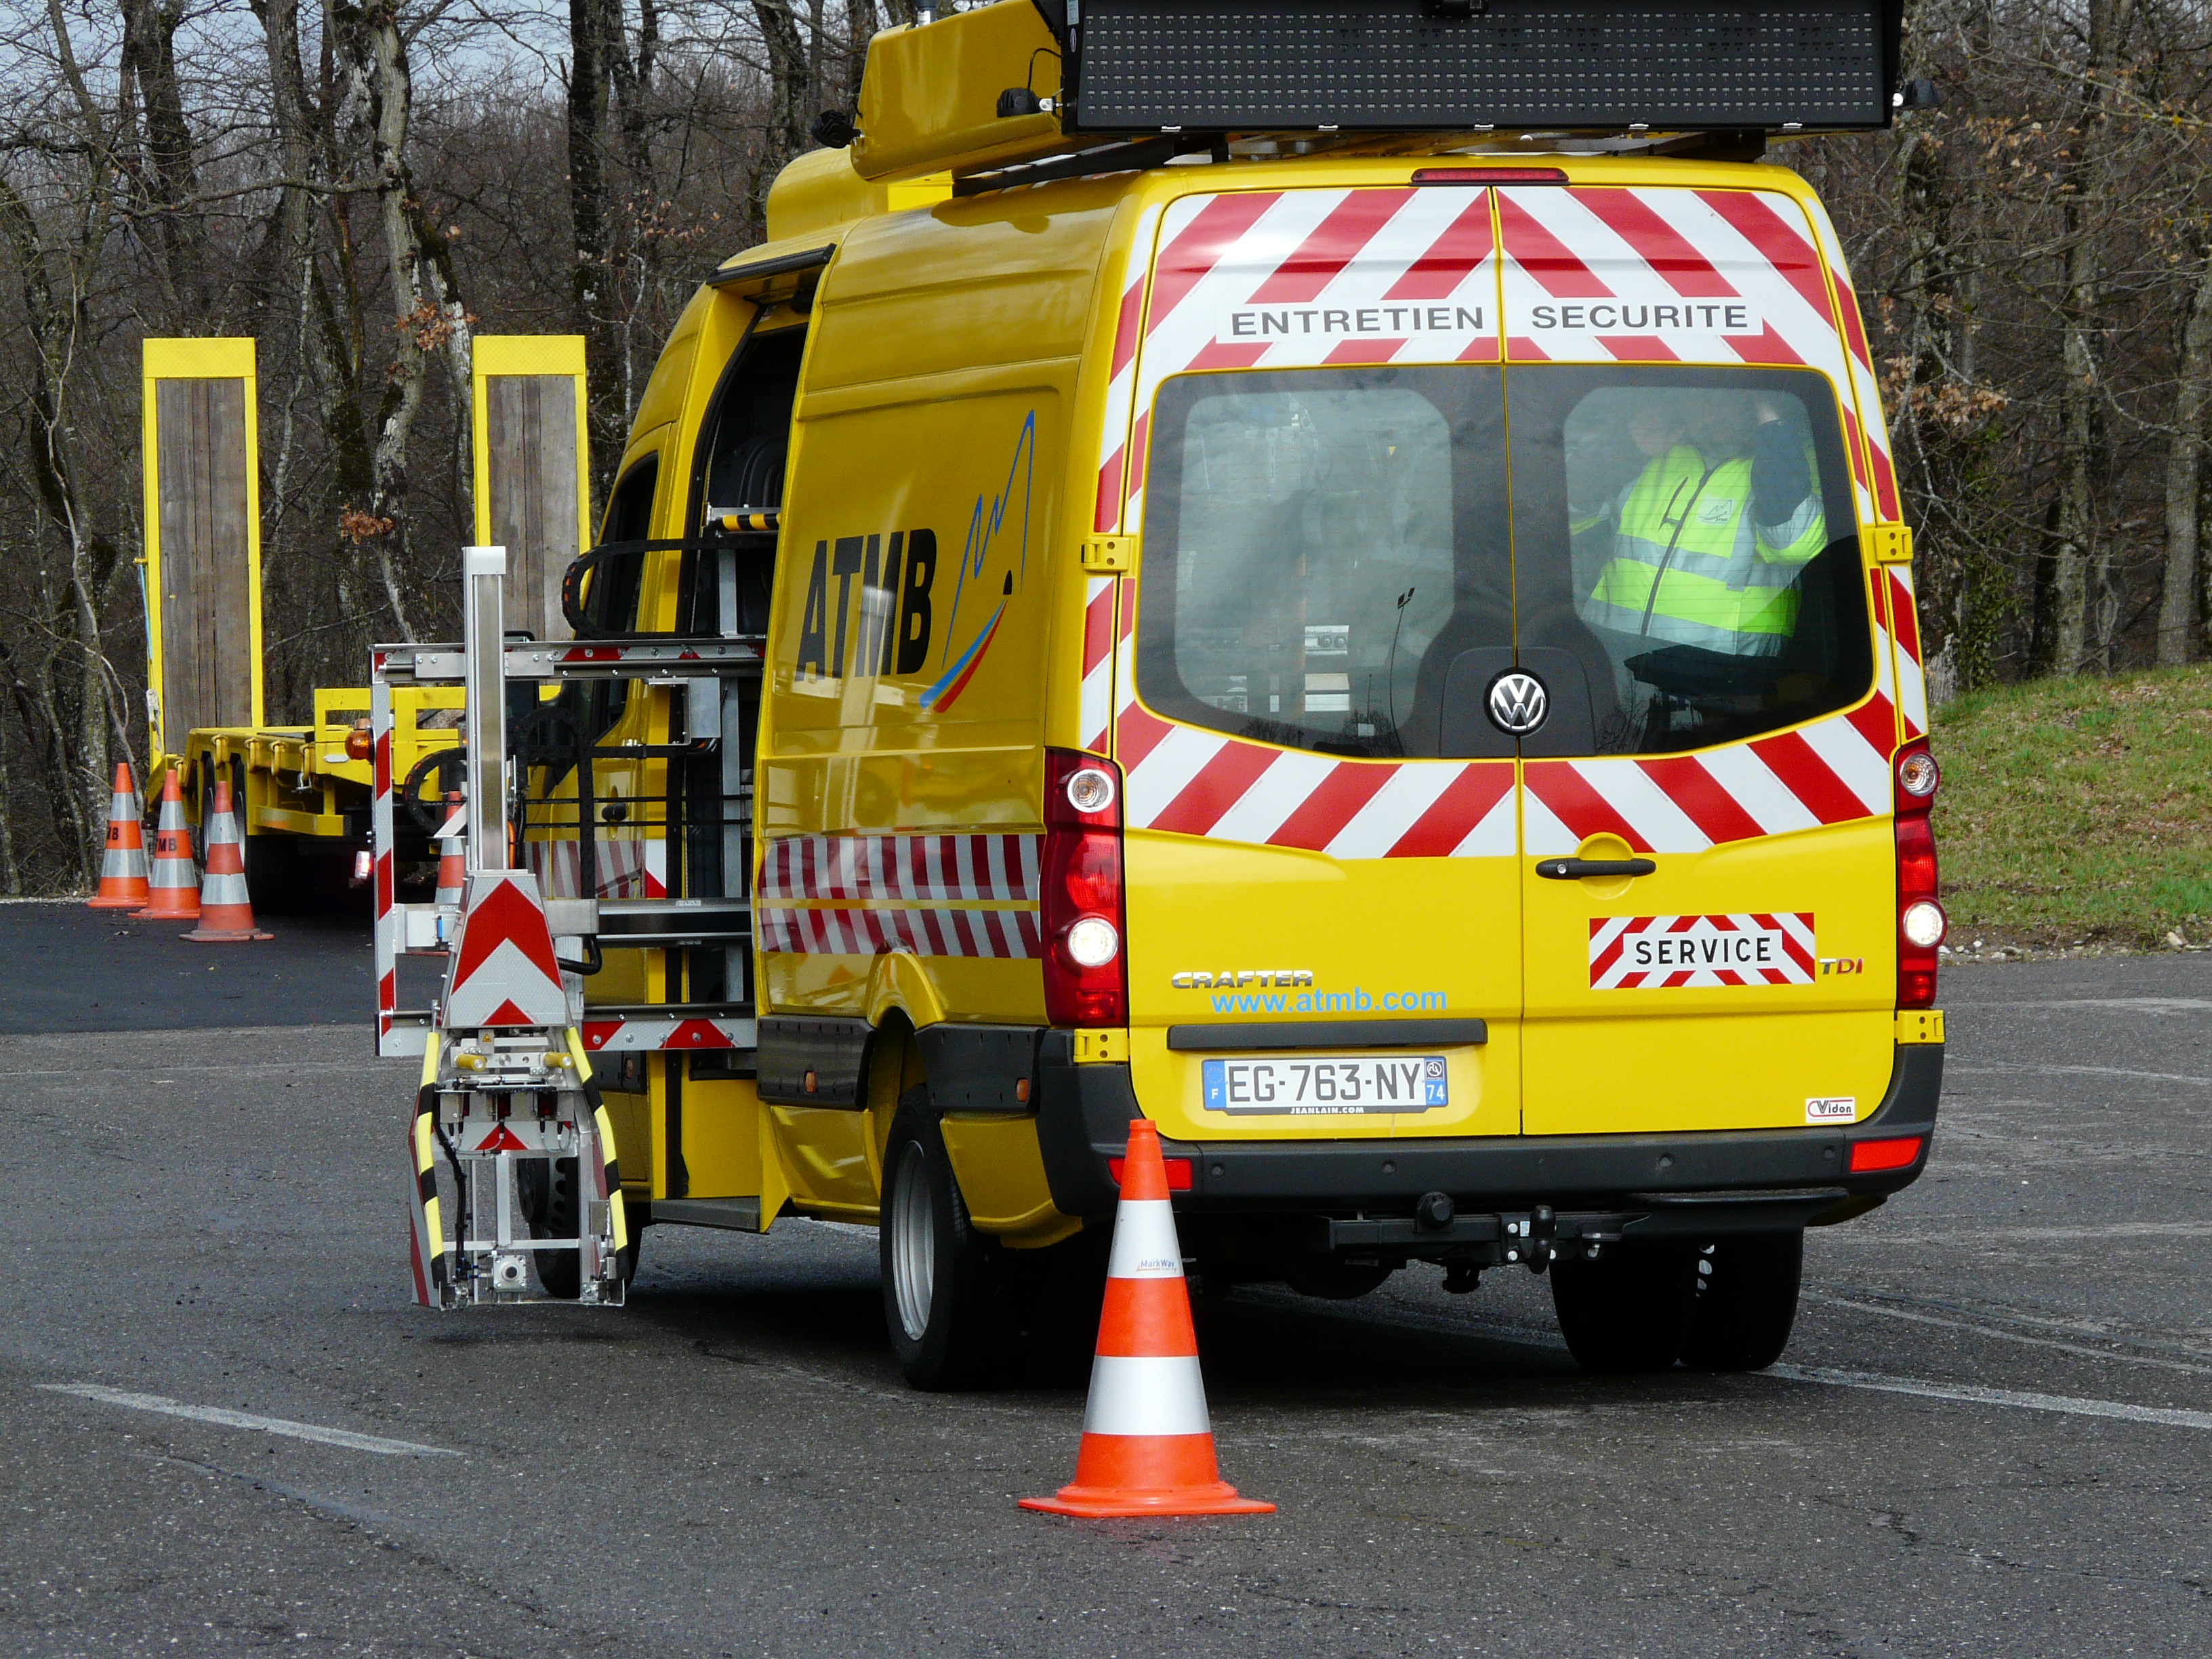
\includegraphics[width=4cm,height=4cm]{images/c4.jpg} \end{subfigure}
        \caption{Véhicules de démonstration modernes}
        \label{fig:vehicules de}
\end{figure}
    
\subsection{Inventaire de signes routiers}

L'inventaire en général se fait dans les villes ou l'environnement est plus complexe que les autoroutes. ils ne sont pas toujours placés perpendiculairement au sol.

\subsection{Systèmes d'assistance aux conducteurs}

Ces systèmes informent ou assistent le conducteur afin d’éviter l’apparition de danger (Figure-\ref{fig:systeme intelligents}).
Il y a des groupes de recherche qui se sont concentrés sur des aspects liés au développement d'un pilote automatique, tels que :
\begin{itemize}
  \item La détection des frontières de la route \cite{3,4} ;
    \item La reconnaissance d'obstacles sur la trajectoire du véhicule tels que d'autres véhicules ou piétons \cite{5,6,7}.
  \end{itemize}
 \vspace{0.5cm} 
 \begin{figure}[h]
        \centering
        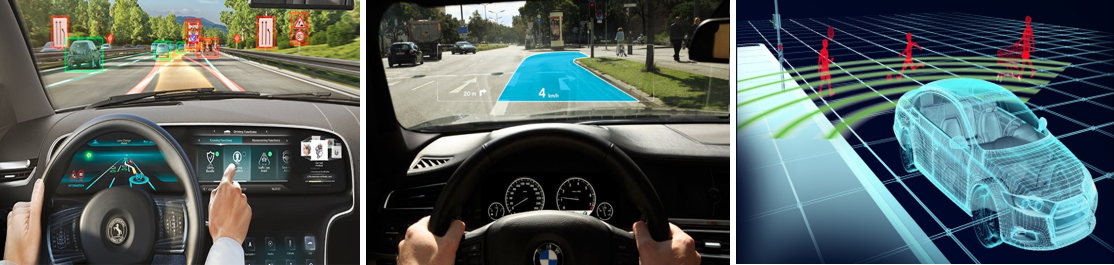
\includegraphics[scale=0.5]{sp.png}
        \caption{Systèmes d'assistance intelligents des voitures}
        \label{fig:systeme intelligents}
\end{figure}
  
\subsection{Véhicules autonomes}

La reconnaissance des panneaux fait partie des fonctions des véhicules autonomes, capable de rouler sans l'intervention d'un conducteur(Figure-\ref{fig:vehicule autonomes}).\\

\begin{figure}[h]
        \centering
        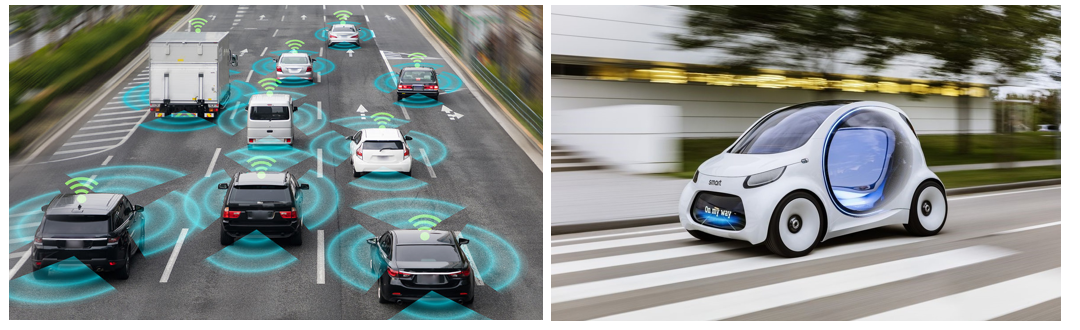
\includegraphics[scale=0.5]{images/tt.png}
        \caption{Véhicules autonomes}
        \label{fig:vehicule autonomes}
\end{figure}
       
\section{Processus de reconnaissance}

Avant de faire la reconnaissance, une étape de détection est d'abord nécessaire (Figure-\ref{fig:processus de}) \cite{10}, ou l’image est pré-traitée, améliorée et segmentée en fonction des propriétés du signe telles que sa couleur ou sa forme. La sortie est une image segmentée contenant des régions potentielles qui pourraient être reconnues comme des panneaux de signalisation possibles.\\

Après cela, vient l’étape de reconnaissance ou chacun des candidats est testé par rapport à un ensemble de fonctionnalités (un modèle) pour décider s’il s’agit ou non d'un panneaux de signalisation, puis selon ces caractéristiques, nous les classons dans différents catégories ou des classes  ou il serait facile de décider de la signification du signe considéré \cite{10}.\\
 
  \begin{figure}[h!]
        \centering
        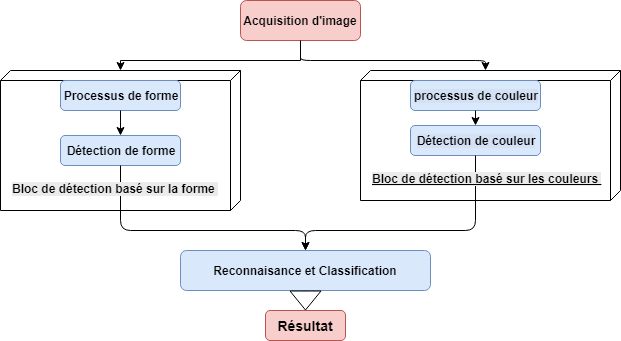
\includegraphics[width=12cm,height=7cm]{yy.png}
        \caption{Processus de détection et de reconnaissance automatique}
        \label{fig:processus de}
\end{figure}
\newpage
Pour mieux expliquer le processus visé par notre travail, la Figure- \ref{fig:schma} présente un schéma typique d’un système de reconnaissance de panneaux routiers. La détection recherche dans les images fournies par une caméra les zones où se trouvent potentiellement des panneaux  (à l’aide d’informations de couleurs, de formes, etc.). Ensuite,un algorithme de reconnaissance permet d’éliminer les régions inutiles et de garder l'information essentielle.\\
\begin{figure}[h]
        \centering
        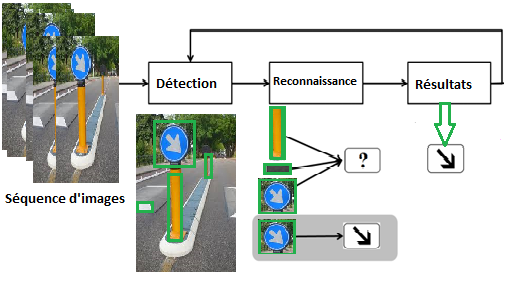
\includegraphics[width=12cm,height=7cm]{images/proces.png}
        \caption{Schéma typique d’un système de reconnaissance}
        \label{fig:schma}
        \end{figure}
\newpage     
\section{Difficultés potentielles  }
Compte tenu de la complexité de l’environnement routier et des scènes qui l'entourent, les panneaux routiers peuvent se trouver dans différentes situations (les exemples de Figure \ref{fig:problemes}), et par conséquent, la détection et la reconnaissance de ces signes peut être entravée par les difficultés suivantes \cite{10} :
\begin{enumerate}
  \item Conditions d’éclairage, qui sont variables et non contrôlables (Figure \ref{fig:problemes} (a),(c));
  \item Présence d'obstacles (Figure \ref{fig:problemes} (d),(e)) ;
  \item L'état physique d'un signe change en fonction de son âge, des accidents, etc (Figure \ref{fig:problemes} (f)) ;
  \item Vu qu’il existent beaucoup de degrés de liberté, la taille de l'objet dépend de la distance à la caméra. l'échelle pour chaque axe est différente (par exemple quand l'axe optique de la caméra n'est pas perpendiculaire au signe), ce qui entraîne une modification de l'aspect de la caméra (Figure \ref{fig:problemes} (g)).
  
 \subsection{Système d'acquisition}
La fonction fondamentale du système d’acquisition est de capturer l'image ou la vidéo afin qu'elle puisse être traitée ultérieurement. La position et la résolution des caméras acquérant les images de signes sont la principale préoccupation. Si les caméras sont placées trop loin (Figure \ref{fig:problemes} (b),(e)), l'image capturée sera floue et si la caméra est placée trop près de la plaque, l'image résultante sera de très grande taille. Par conséquent, la distance entre la caméra et la plaque détermine la qualité de l'image.
 \end{enumerate}
 
 \begin{figure}[h]
        \centering
        \begin{subfigure}
            \centering
            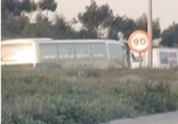
\includegraphics[width=4.2cm,height=4cm]{images/a.png} 
            \caption{(a)}
        \end{subfigure}
        \begin{subfigure}
            \centering
            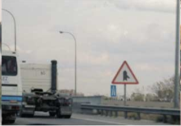
\includegraphics[width=4.2cm,height=4cm]{images/b.png} 
            \caption{(b)}
        \end{subfigure}
        \begin{subfigure}
            \centering
            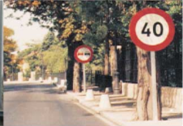
\includegraphics[width=4.2cm,height=4cm]{images/c3.png} 
            \caption{(c)}
        \end{subfigure}
        \begin{subfigure}
            \centering
            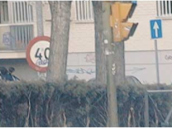
\includegraphics[width=4.2cm,height=4cm]{images/d.png} 
           \caption{(d)}
        \end{subfigure}
        \begin{subfigure}
            \centering
            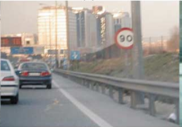
\includegraphics[width=4.2cm,height=4cm]{images/e.png} 
            \caption{(e)}
        \end{subfigure}
        \begin{subfigure}
            \centering
            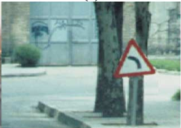
\includegraphics[width=4.2cm,height=4cm]{images/f.png} 
            \caption{(f)}
        \end{subfigure}
        \begin{subfigure}
            \centering
            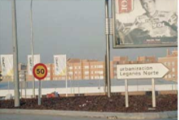
\includegraphics[width=4.2cm,height=4cm]{images/g.png}
            \caption{(g)}
        \end{subfigure}
        \caption{Problèmes rencontrés lors de la  détection et la reconnaissance }
        \label{fig:problemes}
\end{figure}
  \newpage
\section{Conclusion}
Dans ce chapitre, nous avons vu quelques notions fondamentales concernant les classes de panneaux de signalisation routière, les problèmes de normalisation malgré la conventions de Vienne et leurs différents domaines d’application pour montrer l’impact de ce travail et son importance sur la route. Nous avons aussi exposé quelques difficultés qui entravent la détection et la reconnaissance de panneaux de signalisation routière.
%%% Local Variables: 
%%% mode: latex
%%% TeX-master: "../phdthesis"
%%% End: 

% \include{2-chapters/2-3-another-chapter}
% \chapter*{Conclusion et perspectives}
\addstarredchapter{Conclusion}
\markboth{Conclusion}{Conclusion}
\label{sec:conclusion}

   Dans ce travail, nous avons mis en place un système capable de reconnaître automatiquement les panneaux de signalisation routière existant dans une image. Le système effectue la classification des images et détermine la catégorie du
   panneau routier.\\
   La classification des panneaux de signalisation a été effectuée par un réseau de neurone profond de type convolutionnel par rapport à deux architectures différentes(VGGnet et Spatial transformer).\\
   
   Les résultats obtenus montre que l'apprentissage par les données syntde type 'Spatial Transformer Network' donne un taux de reconnaissance meilleur que celle 
   Le problème majeur qu’on a rencontré dans cette partie, est le temps de calcul immense que nécessite l’apprentissage des réseaux de neurones profonds y-compris ceux de type convolutionnel.\\

Les expériences menées dans cette partie ont montrées que l’entraînement sur des données synthétisées donne des résultats améliorés par rapport à celui effectué sur les données réelles dans les deux cas : pour le  ‘VGGnet’ et aussi pour le modèle de « Spatial Transformer network ».
D’un autre coté, les résultats montrent aussi que le modèle de "Spatial Transformer Network" est meilleur que celui du "VGGnet" pour les deux types de data-set.\\

Suite à ce travail, de nombreuses perspectives sont envisageables, les plus importants étant :
\begin{itemize}
    \item Entamer le module de la  de détection qui présente une partie importante dans ce genre de systèmes et explorer ses différentes méthodes tout en effectuant des contributions par rapport à ce qui a était fait déjà dans la littérature;
    \item Pour la reconnaissance, le taux de classification peut être amélioré en enrichissant la base d’apprentissage par d’autres types d’augmentation de données;
    \item L'implémentation de d'autres architechtures de réseaux de neurones et faire des études comparative (Comparative Survey) afin d'avoir une idée globale sur les performances des réseaux de neurones par rapport à la classification des panneaux de signalisation;
    \item Essayer d'exploiter le même travail mais avec des captures vidéos ;
    \item Introduire une fonction de poursuite (faire le suivi) pour déterminer les correspondances entre les images successives. Ceci permettra d’améliorer le temps de détection dans les images qui suivent d’une part et d’améliorer la qualité de la classification d’autre part;
    \item Estimation de la position des panneaux par rapport à la caméra afin de déterminer leur géolocalisation et faciliter ainsi leur gestion et maintien;
    \item Continuer le développement du Benchmark Algérien et investiguer beaucoup plus sur le mauvais taux de classification obtenu.

\end{itemize}






\begin{document}
% Include the title pages
% (the first is made mandatory by UDG and the second is more traditional)
\makeflyleaf

%%% Local Variables: 
%%% mode: latex
%%% TeX-master: "../phdthesis"
%%% End: 


% Build a per-chapter table of content
\dominitoc

% Use roman page numbering for non-significant pages
\pagenumbering{roman}
\frontmatter

% Include the acknowledgements page
\cleardoublepage
\chapter*{Remerciements}
\vspace*{1.5cm}

\begin{center}
    
	
		En premier lieu on tient à présenter nos plus sincères
		
		remerciements et notre profonde reconnaissance à notre  promoteur, \\
		
		le Cne. Amamra Abdenour ; \\
		
		Un exemple à suivre, pour son aide précieuse,
		
		ses conseils et suggestions, 
		
		sa disponibilité et aussi qui a essayé durant toute Cette période,
		
		prise de son précieux temps, 
		
		de nos transmettre les fruits de son
		expérience.\\
		
		On remercie également tous les enseignants qui ont participé à notre
		formation, de près ou de loin.\\
		
		Enfin, on remercie tout le personnel de la brigade élèves, pour
		
		leurs conseils, leurs disponibilité, ainsi que leurs patience et leurs encadrement,
		
		et que tous ceux que nous avons involontairement oublier trouvent ici
		
		l’expression de notre gratitude.

\end{center}

%%% Local Variables: 
%%% mode: latex
%%% TeX-master: "../phdthesis"
%%% End: 


% Build the general table of contents
\setcounter{tocdepth}{2}
\tableofcontents

% Build the list of figures
\listoffigures

% Build the list of tables
\listoftables

% Include the acronym list
%\cleardoublepage
%\chapter*{Table des sigles et acronymes}
\addstarredchapter{Table des sigles et acronymes}
\markboth{Table des sigles et acronymes}{Table des sigles et acronymes}

% Remember to use italic fonts for foreign words
\begin{acronym}[CP-OFDMX] % Specify the longest acronym in order to set the first column width
\acro{3GPP}{\emph{3rd Generation Partnership Project}}
\acro{ADC}{\emph{Analog-to-Digital Conversion}}
\acro{ASK}{\emph{Amplitude Shift Keying}}
\acro{DGA}{Direction Générale de l'Armement}
\end{acronym}

% To cite an acronym in the text : \ac{ASK}
% To cite an acronym in the text without footnote : \acs{ASK}

%%% Local Variables: 
%%% mode: latex
%%% TeX-master: "../phdthesis"
%%% End: 


%%%%%%%%%%%%%%%%%%%%%%%%%%
%%% Chapters are included here %%%
%%%%%%%%%%%%%%%%%%%%%%%%%%

% Use arabic page numbering for significant pages
\mainmatter
\pagestyle{fancy}
%\usepackage{amssymb}
% Include the chapters
\chapter*{Introduction Générale}
\addstarredchapter{Introduction Générale}
\markboth{Introduction}{Introduction}
\label{chap:introduction}
%\minitoc

Le développement technologique rapide a permis aux véhicules de devenir l’un des moyens de transport les plus confortables et fiables. Cependant, des phénomènes alarmants lies à la circulation routière sont apparus tels que la congestion bloquante et les accidents mortels. Chaque année, environ 40.000 personnes meurent sur les routes, et 1,7 millions autres sont grièvement blessées \cite{25}. Autre que les dégâts humains, les coûts annuels engendrés par les accidents de la route s’élèvent à près de 3 \% du PIB mondial, et le problème continue à s’aggraver à cause de la disparité entre le rythme de construction de routes et le nombre de véhicules qui les occupent chaque année. \\

D'autre part, les panneaux de signalisation routière constituent un élément important dans l’organisation et la sécurisation du trafic routier. Leurs respect réduit considérablement le nombre et l’impact des accidents. De nos jours, la disponibilité du matériel et du logiciel performants, ainsi que l’avancement notable dans le domaine d’apprentissage automatique ont rendu possible le développement de systèmes robustes pour la détection et de reconnaissance automatique de panneaux de signalisation routière.  De tels systèmes permettront, par exemple, d’alerter le conducteur de la présence d’un signe de « Stop », de « Sens interdit » dont l’inattention du conducteur peut découler à un dégât mortel. Ce même système est indispensable pour les véhicules autonomes qui sont déjà sur les routes des payes développés. D’autant plus, la reconnaissance automatique des plaques aide dans l’entretien des panneaux défectueux qui est une tache fastidieuse qui doit se faire périodiquement. Pour ces raisons, de tels systèmes attirent de plus en plus l’attention des industriels de l’automobile. Certains modèles de véhicules haut de gamme sont déjà équipés de fonctionnalité de détection automatique des panneaux sans qu’ils soient autonomes. \\

Dans la lumière de cette thématique, nous proposons une étude des algorithmes de reconnaissance des panneaux routiers en utilisant des techniques d’apprentissage profonds ou «\textit{Deep Leanring}». Plus particulièrement, nous nous intéressons aux architectures de réseaux de neurones profonds de type convolutif ou CNN (\textit{Convolutional Neural Networks}) – qui sont mieux adaptés aux taches de classification d’images. Plusieurs variantes de ces modèles seront comparées afin d’établir des choix fondés avant de développer une solution déployable. En plus, nous avons proposé une approche basée sur l’apprentissage a partir de données synthétiques pour remédier aux problèmes de différence d'apparence des signes à travers les pays et a l’insuffisance ou le déséquilibre de la quantité de données d’apprentissage.\\
 
Afin de mieux présenter les techniques étudiées et les résultats obtenus suite au travail effectué, le reste de ce mémoire est organisé en trois parties. Dans la première, nous présentons des généralités sur les panneaux de signalisation routière et leurs normalisations. Nous enchaînons avec des applications du système de reconnaissance automatique et quelques difficultés qui les entravent.

Dans la deuxième partie, divisée en deux chapitres, nous évoquons la détection ainsi que la reconnaissance des panneaux routiers. Nous présentons, d'abord,  l'état de l’art du domaine et les notions relatives a ces deux taches, puis une étude comparative entre les différentes méthodes de reconnaissance est effectuée. 

Nous entamons la troisième partie par un aperçu sur le \emph{Deep Learning} et nous mettons l’accent sur les CNN pour la classification des images. Une étude expérimentale approfondie sera par la suite menée pour montrer les performances de certaines variantes de CNN, en l'occurrence, le  \textbf{VGGnet 16} \cite{simonyan2014very} et \textbf{Inception} \cite{43022} sur les données de panneaux de signalisation routière \textbf{GTRSB} (German Traffic Sign Recognition Benchmark \cite{Stallkamp2012}), sur lesquelles nous avons effectué une étude comparative de leurs performance. Ensuite, et afin de résoudre le problème de quantité de données d'apprentissage nécessaires, nous étudions l'apport de données synthétiques, qui sont  plus faciles à obtenir et a manipuler.\\ 

Nous clôturons ce mémoire par une conclusion générale ou nous résumons les travaux que nous avons effectues et nous citerons quelques perspectives dans l'objectif de l’améliorer et d'orienter futurs travaux sur la même problématique.





 

%%% Local Variables: 
%%% mode: latex
%%% TeX-master: "../phdthesis"
%%% End: 

\part{Concepts Fondamentaux }
\chapter{Reconnaissance des panneaux de signalisation routière}
\label{chap:premierchapitre}
\minitoc

Dans ce chapitre, nous allons voir des généralités sur les panneaux de signalisation routière ainsi que différentes applications des systèmes de détection et de reconnaissance automatiques tout en entamant les étapes principales du processus de la reconnaissance.

\section{Panneaux de signalisation routière}

Les panneaux de signalisation routière constituent un élément important de la circulation routière. Leur fonction principale est d’exposer et d’afficher le contenu qui doit avertir les conducteur des dangers potentiels ainsi que les informations sur la route. C’est pour cette raison que la détection et l’identification des panneaux de signalisation est un aspect de recherche très important dans la prévention des accidents au niveau de route (Figure- \ref{fig: panneaux-al}).

\begin{figure}[htp!]
     \centering
      \begin{subfigure}
          \centering    
              
\includegraphics[width=3.5cm,height=4cm]{images/ii.jpg}
              \end{subfigure}
           \hfill
     \begin{subfigure}
              \centering  
       
\includegraphics[width=3.5cm,height=4cm]{images/300.jpg}
     \end{subfigure}
          \hfill
     \begin{subfigure}
             \centering     
            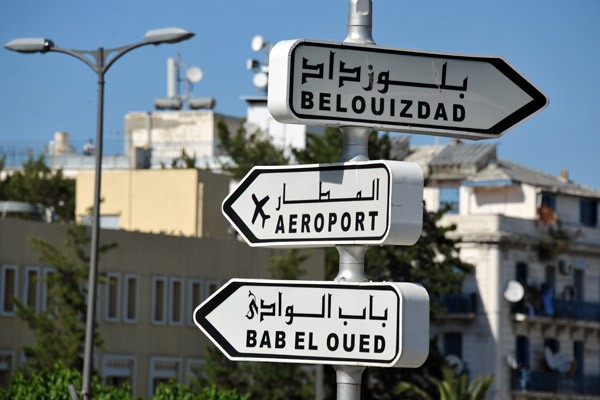
\includegraphics[width=3.5cm,height=4cm]{images/3.jpg}
     \end{subfigure}
           \hfill
     \begin{subfigure}
              \centering    
            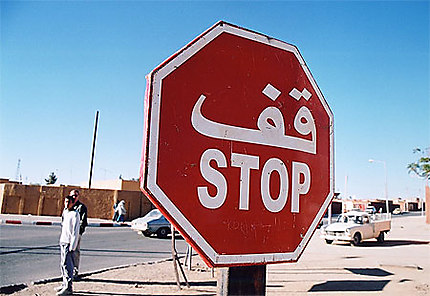
\includegraphics[width=3.5cm,height=4cm]{images/5.jpg}
     \end{subfigure}
      \caption{Exemples de plaques routières en Algérie}
       \label{fig: panneaux-al}
\end{figure}

\subsection{Classification des panneaux de signalisation routière }

Une convention sur la signalisation routière a été faite à Vienne le 8 novembre 1968. Cette dernière consiste en un  traité international qui a réuni un ensemble de pays (Figure- \ref{fig:participants de Viennes}), reconnaissant que l’uniformité et la normalisation des panneaux de signalisation, des feux de circulation de routes et des marquages, sont nécessaires pour gérer la circulation routière. \cite{1}.\\

\begin{figure}[h!]
        \centering
        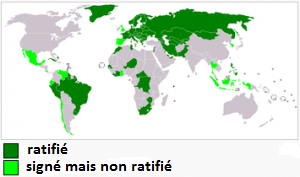
\includegraphics[width=8cm,height=4cm]{images/vienna.png}
        \caption{Participants à l’union de Vienne}
        \label{fig:participants de Viennes}
\end{figure}
    
A partir de cette réunion, plusieurs  articles ont été fournis parmi lesquelles l’article numéro "02" qui classe les panneaux de signalisation routière en catégories nommées de ‘A’  à ‘H’ contenant chacune un groupe de panneaux spécifiques (Tableau-\ref{table:classes de panneaux}).\\
Les sections principales issues de l’article sont:
\begin{table}[]
\centering
\begin{tabular}{|l|l|l|}
\hline
\multicolumn{1}{|c|}{code de la section} & \multicolumn{1}{|c|}{contenu} & \multicolumn{1}{|c|}{exemple}  \\ \hline
  \multicolumn{1}{|c|}{A }
  & 
  \multicolumn{1}{|c|}{Les panneaux d'avertissement de danger} 
  & 
 \multicolumn{1}{|c|}{
\includegraphics[width=2.5cm,height=2cm]{100.jpg}}   \\ \hline
  \multicolumn{1}{|c|}{B}    &
\multicolumn{1}{|c|}{Les signes de priorité} 
& \multicolumn{1}{|c|}{
\includegraphics[width=2.5cm,height=2cm]{101.jpg}} \\ \hline
 \multicolumn{1}{|c|}  {C}  
    & 
 \multicolumn{1}{|c|}   {Les signes d'interdiction ou de restriction}   & 
 \multicolumn{1}{|c|}  {
\includegraphics[width=2.5cm,height=2cm]{102.jpg} }\\ \hline
     \multicolumn{1}{|c|} {D} 
    & 
    \multicolumn{1}{|c|}{Les signes obligatoires}
    & 
     \multicolumn{1}{|c|} {
\includegraphics[width=2.5cm,height=2cm]{103.png}}  \\ \hline
      \multicolumn{1}{|c|}{E}  
    & 
    \multicolumn{1}{|c|}{Signalisation réglementaire spéciale}  
    & 
 \multicolumn{1}{|c|} {
\includegraphics[width=2.5cm,height=2cm]{sss.png}} \\  \hline  
  \multicolumn{1}{|c|} {F}   
    & 
    \multicolumn{1}{|c|}{Informations, installations ou panneaux de service} 
    & 
    \multicolumn{1}{|c|}{
\includegraphics[width=2.5cm,height=2cm]{exit.png}} \\      \hline 
   \multicolumn{1}{|c|}{G}
    & 
   \multicolumn{1}{|c|} {Panneau de direction, de position ou d'indication}
    & 
   \multicolumn{1}{|c|}{
\includegraphics[width=2.5cm,height=2cm]{104.jpg}} \\       \hline   
   \multicolumn{1}{|c|}{H } 
    & 
    \multicolumn{1}{|c|}{Panneaux supplémentaires} 
    & 
    \multicolumn{1}{|c|}{
\includegraphics[width=2.5cm,height=2cm]{images/200.png}} \\  \hline   
         
\end{tabular}
\caption{Classes de panneaux de signalisation routière}
\label{table:classes de panneaux}
\end{table}
\newpage
La convention, dans une deuxième partie, définit les couleurs, des tailles et des formes précises pour chacune de ces classes de signes.\\
Malgré les normalisations et les standards qui furent révisés plusieurs fois, il existe toujours des différences entre les pays contractés dans l’accord. Le tableau (Table-\ref{table:diff-p}) montre des panneaux indiquant la présence d'un passage piéton dans différents pays.\\
\begin{table}[]
\centering
\begin{tabular}{|l|l|l|}
\hline
\multicolumn{1}{|c|}{
\includegraphics[width=3cm,height=2.5cm]{images/pieton5.png}} & \multicolumn{1}{c|}{
\includegraphics[width=3cm,height=2.5cm]{images/pieton3.png}} & \multicolumn{1}{c|}{
\includegraphics[width=3cm,height=2.5cm]{images/pieton3.png}} \\ \hline
\multicolumn{1}{|c|}{En Malaisie}    & \multicolumn{1}{c|}{Au Japon }  & \multicolumn{1}{c|}{Aux Philippines}\\ \hline
\end{tabular}
\caption{Exemple de différence entre les panneaux de         signalisation routière}
\label{table:diff-p}
\end{table}
\subsection{Propriétés des panneaux de signalisations routière}

Les panneaux de signalisation ont été conçus pour être distincts des arrières plans naturels ou artificiels et ils ont des caractéristiques qui les rendent reconnaissables dans l’environnement. En général, ils sont fabriqués et installés conformément à des règles strictes (Figure- \ref{fig:formes}).
Les symboles sur les panneaux ont une couleur qui les distingue de l'arrière plan de la scène. La teinte de la peinture qui recouvre le signe correspond à une longueur d'onde spécifique dans le spectre visible. Les panneaux sont situés à des emplacements bien définis sur la route, de sorte que le conducteur peut s’attendre à les observer. Ils  peuvent contenir des pictogrammes, du texte ou les deux au même temps tout en prenant une forme géométrique particulière (cercle,triangle, rectangle, etc.)
\begin{figure}[h]
  \centering
  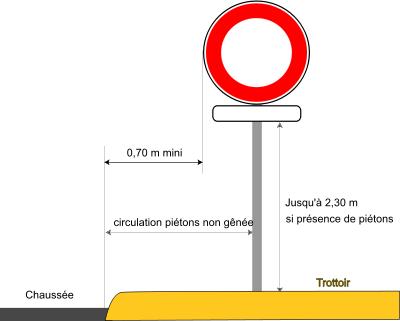
\includegraphics[width=7cm,height=5cm]{images/rte.png}
  \caption{Exemple de différentes règles d'implantations d'un panneau routier}
  \label{fig:formes}
\end{figure}

\newpage
\section{Domaines d’application}

La détection et la reconnaissance des panneaux de signalisation routière a prouvée un grand intérêt au cours des dernières années,cela est dû au large éventail d'applications qu'un système doté de cette capacité offre;

\subsection{Entretien des autoroutes}

Quotidiennement, un opérateur humain doit  vérifier la présence et l'état des panneaux au niveau des autoroutes (Figure-\ref{fig:entretien}).\\

\begin{figure}[h]
        \centering
        \includegraphics[width=10cm,height=3cm]{images/ccc.png}
        \caption{Entretien de panneaux routiers}
        \label{fig:entretien}
\end{figure}

C'est une tâche fastidieuse car les panneaux sont nombreux. Il y a un projet européen appelé "AUTOCAT" \cite{2} qui présente une fourgonnette développée pour la collecte automatique de la position et l'orientation des panneaux de signalisation routière (Figure- \ref{fig:vehicules de}) ci-dessus montre des véhicules modernes dans le même contexte.

\begin{figure}[h]
        \centering
        \begin{subfigure}
        \centering
        \includegraphics[width=4cm,height=4cm]{images/c1.png}  \end{subfigure}
         \begin{subfigure}
         \centering
        \includegraphics[width=4cm,height=4cm]{images/c2.png}
        \end{subfigure}
        \begin{subfigure}
        \centering
        \includegraphics[width=4cm,height=4cm]{images/c4.jpg} \end{subfigure}
        \caption{Véhicules de démonstration modernes}
        \label{fig:vehicules de}
\end{figure}
    
\subsection{Inventaire de signes routiers}

L'inventaire en général se fait dans les villes ou l'environnement est plus complexe que les autoroutes. ils ne sont pas toujours placés perpendiculairement au sol.

\subsection{Systèmes d'assistance aux conducteurs}

Ces systèmes informent ou assistent le conducteur afin d’éviter l’apparition de danger (Figure-\ref{fig:systeme intelligents}).
Il y a des groupes de recherche qui se sont concentrés sur des aspects liés au développement d'un pilote automatique, tels que :
\begin{itemize}
  \item La détection des frontières de la route \cite{3,4} ;
    \item La reconnaissance d'obstacles sur la trajectoire du véhicule tels que d'autres véhicules ou piétons \cite{5,6,7}.
  \end{itemize}
 \vspace{0.5cm} 
 \begin{figure}[h]
        \centering
        \includegraphics[scale=0.5]{sp.png}
        \caption{Systèmes d'assistance intelligents des voitures}
        \label{fig:systeme intelligents}
\end{figure}
  
\subsection{Véhicules autonomes}

La reconnaissance des panneaux fait partie des fonctions des véhicules autonomes, capable de rouler sans l'intervention d'un conducteur(Figure-\ref{fig:vehicule autonomes}).\\

\begin{figure}[h]
        \centering
        \includegraphics[scale=0.5]{images/tt.png}
        \caption{Véhicules autonomes}
        \label{fig:vehicule autonomes}
\end{figure}
       
\section{Processus de reconnaissance}

Avant de faire la reconnaissance, une étape de détection est d'abord nécessaire (Figure-\ref{fig:processus de}) \cite{10}, ou l’image est pré-traitée, améliorée et segmentée en fonction des propriétés du signe telles que sa couleur ou sa forme. La sortie est une image segmentée contenant des régions potentielles qui pourraient être reconnues comme des panneaux de signalisation possibles.\\

Après cela, vient l’étape de reconnaissance ou chacun des candidats est testé par rapport à un ensemble de fonctionnalités (un modèle) pour décider s’il s’agit ou non d'un panneaux de signalisation, puis selon ces caractéristiques, nous les classons dans différents catégories ou des classes  ou il serait facile de décider de la signification du signe considéré \cite{10}.\\
 
  \begin{figure}[h!]
        \centering
        \includegraphics[width=12cm,height=7cm]{yy.png}
        \caption{Processus de détection et de reconnaissance automatique}
        \label{fig:processus de}
\end{figure}
\newpage
Pour mieux expliquer le processus visé par notre travail, la Figure- \ref{fig:schma} présente un schéma typique d’un système de reconnaissance de panneaux routiers. La détection recherche dans les images fournies par une caméra les zones où se trouvent potentiellement des panneaux  (à l’aide d’informations de couleurs, de formes, etc.). Ensuite,un algorithme de reconnaissance permet d’éliminer les régions inutiles et de garder l'information essentielle.\\
\begin{figure}[h]
        \centering
        \includegraphics[width=12cm,height=7cm]{images/proces.png}
        \caption{Schéma typique d’un système de reconnaissance}
        \label{fig:schma}
        \end{figure}
\newpage     
\section{Difficultés potentielles  }
Compte tenu de la complexité de l’environnement routier et des scènes qui l'entourent, les panneaux routiers peuvent se trouver dans différentes situations (les exemples de Figure \ref{fig:problemes}), et par conséquent, la détection et la reconnaissance de ces signes peut être entravée par les difficultés suivantes \cite{10} :
\begin{enumerate}
  \item Conditions d’éclairage, qui sont variables et non contrôlables (Figure \ref{fig:problemes} (a),(c));
  \item Présence d'obstacles (Figure \ref{fig:problemes} (d),(e)) ;
  \item L'état physique d'un signe change en fonction de son âge, des accidents, etc (Figure \ref{fig:problemes} (f)) ;
  \item Vu qu’il existent beaucoup de degrés de liberté, la taille de l'objet dépend de la distance à la caméra. l'échelle pour chaque axe est différente (par exemple quand l'axe optique de la caméra n'est pas perpendiculaire au signe), ce qui entraîne une modification de l'aspect de la caméra (Figure \ref{fig:problemes} (g)).
  
 \subsection{Système d'acquisition}
La fonction fondamentale du système d’acquisition est de capturer l'image ou la vidéo afin qu'elle puisse être traitée ultérieurement. La position et la résolution des caméras acquérant les images de signes sont la principale préoccupation. Si les caméras sont placées trop loin (Figure \ref{fig:problemes} (b),(e)), l'image capturée sera floue et si la caméra est placée trop près de la plaque, l'image résultante sera de très grande taille. Par conséquent, la distance entre la caméra et la plaque détermine la qualité de l'image.
 \end{enumerate}
 
 \begin{figure}[h]
        \centering
        \begin{subfigure}
            \centering
            \includegraphics[width=4.2cm,height=4cm]{images/a.png} 
            \caption{(a)}
        \end{subfigure}
        \begin{subfigure}
            \centering
            \includegraphics[width=4.2cm,height=4cm]{images/b.png} 
            \caption{(b)}
        \end{subfigure}
        \begin{subfigure}
            \centering
            \includegraphics[width=4.2cm,height=4cm]{images/c3.png} 
            \caption{(c)}
        \end{subfigure}
        \begin{subfigure}
            \centering
            \includegraphics[width=4.2cm,height=4cm]{images/d.png} 
           \caption{(d)}
        \end{subfigure}
        \begin{subfigure}
            \centering
            \includegraphics[width=4.2cm,height=4cm]{images/e.png} 
            \caption{(e)}
        \end{subfigure}
        \begin{subfigure}
            \centering
            \includegraphics[width=4.2cm,height=4cm]{images/f.png} 
            \caption{(f)}
        \end{subfigure}
        \begin{subfigure}
            \centering
            \includegraphics[width=4.2cm,height=4cm]{images/g.png}
            \caption{(g)}
        \end{subfigure}
        \caption{Problèmes rencontrés lors de la  détection et la reconnaissance }
        \label{fig:problemes}
\end{figure}
  \newpage
\section{Conclusion}
Dans ce chapitre, nous avons vu quelques notions fondamentales concernant les classes de panneaux de signalisation routière, les problèmes de normalisation malgré la conventions de Vienne et leurs différents domaines d’application pour montrer l’impact de ce travail et son importance sur la route. Nous avons aussi exposé quelques difficultés qui entravent la détection et la reconnaissance de panneaux de signalisation routière.
%%% Local Variables: 
%%% mode: latex
%%% TeX-master: "../phdthesis"
%%% End: 

\part{ Motivations et État de l’Art}
\label{chap:deuxiemme}

\chapter{Détection des panneaux de signalisation}
\minitoc
\section{Introduction}
Dans cette partie, nous présentons le premier module du système de reconnaissance de panneaux, qui est, la détection tout en entamant quelques fondements ainsi que les différentes techniques et méthodes utilisées.

\section{Détection de panneaux de signalisation}

La phase de détection se base sur l’attention visuelle \cite{11} et comme on a expliqué précédemment, elle utilise des caractéristiques intrinsèques aux panneaux routiers considérés pour détecter les zones de l’image susceptibles de contenir de panneaux routiers.\\

D’abord les caractéristiques visuelles sont extraites de l’image de la scène. Ensuite, les caractéristiques sont combinées pour donner naissance à une carte d’attention visuelle (FOCUS OF INTENTION) qui met en évidence les zones qui peuvent contenir des panneaux routiers .\\
La phase finale de ce module consiste à sélectionner ces zones d’intérêt et les classifier.Pour détecter la position des signes routiers dans les images, nous devons connaître les deux propriétés dont nous avons parlé auparavant (chapitre précédent), à savoir la couleur et la forme.\\

\subsection{Détection basée sur la couleur}

La segmentation des couleurs implique soit l’utilisation du seuillage de couleur ou l'une des méthodes d'apprentissage des couleurs.\\ 

{\textbf{Techniques basées sur le seuillage de couleurs (Color thresholding) }}\\

Les techniques de détection basées sur les couleurs visent à effectuer une recherche dans la zone d'intérêt en fonction des couleurs d'intérêt à l'aide de techniques de seuillage ou de segmentation. Différents espaces colorimétriques peuvent être utilisés pour détecter la couleur d'intérêt et la séparer de l'arrière-plan.\\ Plusieurs modèles ont été conçus,dans les années 1990, plusieurs chercheurs ont utilisé le modèle d'espace colorimétrique Hue-Saturation-Intensity (HSI) \cite{12} et d'autres comme dans \cite{13} ont utilisé le seuillage de couleurs pour segmenter l'image (Figure-\ref{fig:seuillage de couleur}).

\begin{figure}[h]
      \centering
      \begin{subfigure}
      \centering
      \includegraphics[width=4cm,height=4cm]{images/m06y4.jpg}
      \end{subfigure}
      \begin{subfigure}
      \centering
      \includegraphics[width=4cm,height=4cm]{images/111.png}
      \end{subfigure}
    \caption{Exemple de seuillage de couleur rouge}
    \label{fig:seuillage de couleur}
\end{figure}

Alors que les chercheurs dans \cite{14} ont effectué la détection de couleur dans l'espace colorimétrique HSV (hue, saturation, value) et ils ont conclu que la saturation des couleurs varie considérablement lorsque les captures sont prises à partir de différents appareils. Certains d'autres \cite{15} ont étudié l'effet de la lumière sur la couleur des panneaux de signalisation pendant le jour et la nuit et ils ont conclu que la couleur de l'image pouvait être déformée par la lumière et que cela pouvait affecter la qualité des images (figure-\ref{fig:val rgb}).

\begin{figure}[h]
      \centering
    \includegraphics[width=8cm,height=4cm]{images/rgb.png}
    \caption{Valeur RGB en fonction du temps pour un pixel de signe STOP rouge \cite{15} }
    \label{fig:val rgb}
\end{figure}
{\textbf{Techniques basées sur des méthodes d'apprentissage de couleurs}}\\

Il existe plusieurs méthodes d'apprentissage de couleurs qui ont été mises en œuvre pour les panneaux de signalisation.\\
Les auteurs dans \cite{16} ont été les premiers, qui ont travaillé dans le domaine de l'algorithme génétique (GA) pour la détection de signes routiers, Ils ont détecté les panneaux de limitation de vitesse qui ont une forme ronde en utilisant un filtre de lissage et un filtre Laplacien pour éliminer le bruit, puis un algorithme génétique pour la détection de signes (figure-\ref{fig:GA}).\\

\begin{figure}[h]
      \centering
      \includegraphics[width=10cm,height=7cm]{images/uu.png}
    \caption{Processus de détection en utilisant l'algorithme génitique (GA)\cite{16} }
    \label{fig:GA}
\end{figure}

Il y a aussi des algorithmes qui sont basés sur des machines à vecteurs de support (SVM),ce dernier a été proposé par les auteurs dans \cite{17} afin de classer les pixels en se référant sur les informations de couleurs, par contre Dans \cite{18}, les signes sont détectés à l'aide d'un ensemble de caractéristiques en ondelettes de Haar obtenues grâce à l'algorithme AdaBoost.\\
Les auteurs qui ont utilisé ces méthodes d’apprentissage de couleurs  ont conclu que cette dernière donne de meilleurs résultats par rapport à la segmentation par seuillage de couleur.
\subsection{ Détection basée sur la forme}

Les techniques de détection basées sur les couleurs ne sont utiles que si nous utilisons une caméra couleur de haute résolution et elle ne serait pas efficace dans toutes les conditions d’éclairage (la nuit ,les nuages…etc).\\
D’autre part,la détection peut aussi être faite par forme où il en existe plusieurs.\\

{\textbf{Détection de forme à l'aide des bords }}\\

Les techniques de détection de contour dépendent du contour des panneaux. Les auteurs dans \cite{19} ont effectué la détection de signes en utilisant un algorithme de correspondance de motifs rectangulaires simples.\\ 
Alors que d’autres comme par exemple \cite{20} ont utilisé l'équation d'ellipse pour détecter le cercle dans une image.
Cependant, la détection de forme à l'aide de fonctions périphériques ne peut donner des résultats précis que pendant la journée.\\

{\textbf{Détection de forme à l'aide d'une correspondance de modèle}}\\

Cette  méthode en général se base sur l’association entre l'image capturée et les  images de panneaux de signalisation routière de bonne qualité connus dans la base de données.\\ 
L’avantage principal de l’utilisation de cette méthode est qu’elle peut être modifiée pour détecter n’importe quel objet comme dans \cite{21} où « heldon.W et Oruklu » ont appliqué cette technique à l'appariement d'objets.\\

{\textbf{Détection basée sur des techniques d'apprentissage automatiques}}\\

Il y a diverses algorithmes qui peuvent être utilisés pour extraire la forme tels que les machines à vecteurs de support (SVM) et les réseaux de neurones (NN) qui sont les plus utilisés pour la détection de signes en raison de leurs capacité à détecter les formes avec précision.Cependant, concernant les réseaux de neurones, l’ajout de nouveau signes implique à nouveau la formation du réseau.\\ 
D’autres utilisent Les MSER (maximally stable extremal regions) comme dans \cite{21} qui fonctionnent sur les symboles de circulation avec un fond blanc dans laquelle les régions candidates sont détectées comme étant des régions extrêmes à stabilité maximale (MSER) ensuite les caractéristiques de l'histogramme des gradients orientés (HOG) sont dérivés.\\

{\textbf{Détection de forme basée sur la transformation de Hough (HT)}}\\

La transformation de "Hough" est utilisée pour détecter les cercles et les lignes sur la base d'un algorithme d'ajustement de courbes (Figure-\ref{fig:ht}).\\

Les auteurs dans \cite{22} se basent sur l'utilisation de la transformée de Hough standard afin de détecter la forme de la plaque de signalisation routière (par exemple circulaire, carrée, triangulaire,etc).
\begin{figure}[h]
      \centering
      \includegraphics[width=16cm,height=4cm]{rt.png}
    \caption{Processus de détection proposé par \cite{22} en se basant sur Hough transform, SHT:Standard HT, GHT:Generalized HT.}
    \label{fig:ht}
\end{figure}

\section{Conclusion}

À partir de ce chapitre, on a eu une idée générale sur la phase de détection et ces techniques générales les plus utilisées, pour pouvoir constater l'importance de cette étape incontournable par rapport a un système de reconnaissance, tout en parcourant quelques travaux réalisés dans ce contexte.

\chapter{Reconnaissance des panneaux de signalisation}
\minitoc
\section{Introduction}
Une fois la première partie du système de reconnaissance qui est la détection est vu dans le chapitre précédent, Cette partie va être consacrée à la phase de reconnaissance elle-même ( qui est justement notre intérêt de travail), et les techniques utilisées pour réaliser un tel système tout en parcourant quelques travaux connexes concernant cette dernière.

\section{Reconnaissance des panneaux de signalisation}

Le résultat de l’étape de détection est une liste d’objets candidats qui pourraient être des panneaux de signalisation probables. Cette liste est transmise au dispositif de reconnaissance pour une évaluation ultérieure ensuite une classification afin de décider si les objets de la liste sont des objets rejetés ou des panneaux de signalisation en plus de leurs classes de décision.

\subsection{Caractéristiques d’un bon dispositif de reconnaissance }

Pour concevoir un bon système de reconnaissance, de nombreux paramètres doivent être pris en compte.

\begin{enumerate}
\item Le dispositif de reconnaissance doit présenter un bon pouvoir discriminant et un faible coût de calcul;
\item Il doit être robuste à l’état géométrique du signe, tel que l’orientation, la taille et la position du signe dans l’image;
\item Il doit être robuste au bruit;
\item La reconnaissance devrait être effectuée rapidement ;
\item Le classifieur doit pouvoir apprendre un grand nombre de classes d’où il vaut mieux utiliser autant que possible des connaissances a priori sur les panneaux de signalisation.
\end{enumerate}

\subsection{Défis du processus de la  reconnaissance des images}

D’un autre côté, il existe plusieurs défis qui opposent l’opération de la reconnaissance, une liste (non-exhaustive) de certaines difficultés est :
\begin{enumerate}
\item 
\begin{flushleft}
    
    Variation du point de vue\end{flushleft} Une seule instance d'un objet peut être orientée de plusieurs manières par rapport à la caméra(Figure-\ref{fig:variation});
    \begin{figure}[h]
      \centering
      \includegraphics[width=12cm,height=3cm]{images.jpg}
    \caption{Exemple de variation de point de vue d'un panneau routier.}
    \label{fig:variation}
\end{figure}
 \pagebreak   
\item \begin{flushleft} Variation d'échelle\end{flushleft} Les classes visuelles présentent souvent des variations de tailles (Figure-\ref{fig:variation echel}) ;
 \begin{figure}[h!]
      \centering
      \includegraphics[width=10cm,height=4cm]{scale.png}
    \caption{Exemple de variation d'échelle pour un panneau routier représentant "travaux en cours".}
    \label{fig:variation echel}
\end{figure}
\item \begin{flushleft} Déformation\end{flushleft} De nombreux objets d'intérêt ne sont pas des corps rigides ou avec le facteur de l’âge peuvent être déformés de manière extrême (Figure-\ref{fig:deform});
\begin{figure}[h!]
      \centering
      \includegraphics[width=5cm,height=3cm]{defo.jpg}
    \caption{Exemple de déformation d'un panneau routier}
    \label{fig:deform}
\end{figure}
\item \begin{flushleft} Occlusion\end{flushleft} Les objets d'intérêt peuvent être occultés. Parfois, seule une petite partie d'un objet peut être visible (Figure-\ref{fig:occlusion});
\begin{figure}[h]
      \centering
      \includegraphics[width=14cm,height=4cm]{im.jpg}
    \caption{Exemple de panneaux routiers occultés.}
    \label{fig:occlusion}
\end{figure}
\newpage
\item  \begin{flushleft} Conditions d'éclairage\end{flushleft}Les effets de l'illumination ont une grande influence au niveau des pixels (Figure-\ref{fig:conditions});
\begin{figure}[h]
      \centering
      \includegraphics[width=8cm,height=4cm]{ec.jpg}
    \caption{Exemple d'effets d'éclairage sur un panneau routier.}
    \label{fig:conditions}
\end{figure}
\item \begin{flushleft} Fond désordonné\end{flushleft} Les objets d'intérêt peuvent se fondre dans leur environnement, ce qui les rend difficiles à identifier(Figure-\ref{fig:fond});
\begin{figure}[h!]
      \centering
      \includegraphics[width=8cm,height=5cm]{img.jpg}
    \caption{Exemple d'un fond désordonné.}
    \label{fig:fond}
\end{figure}
\pagebreak
\item  \begin{flushleft} Variation intra-classe \end{flushleft}
Les classes d'intérêt peuvent souvent être relativement larges, telles qu’il existe de nombreux types différents de ces objets, chacun ayant sa propre apparence (Figure \ref{fig:intraclasse}) .

\begin{figure}[h!]
      \centering
      \includegraphics[width=8cm,height=4cm]{tl.png}
    \caption{Exemple de variation de plaques dans la même classe.}
    \label{fig:intraclasse}
\end{figure}
\end{enumerate}

Un bon système de reconnaissance des images doit être invariant pour le produit croisé de toutes ces variations,tout en conservant la sensibilité aux variations entre les classes.

\section{Méthodes de Reconnaissance }

Il existe plusieurs techniques utilisés pour la phase de reconnaissance dont on cite : K-plus proche voisin (K-nearest neighbor),Groupements de K-moyennes (K-mean clustering), Classifieur linéaire,Machines à vecteur de support(SVM) et les réseaux de neurones.

\subsection{Classifieur du voisin le plus proche (K-nearest neighbor) }

Ce classifieur prend une image test,et la compare à chacune des images d'apprentissage et prédit l'étiquette de l'image d'apprentissage la plus proche.\\
La notion de K-voisins plus proches présente une idée très simple: au lieu de trouver l'image la plus proche unique dans l'ensemble de formation, nous allons rechercher les k premières images les plus proches et les faire voter sur l'étiquette de l'image test. En particulier, lorsque k = 1, nous récupérons le classificateur  du voisin le plus proche.\\ Intuitivement, les valeurs élevées de k ont un effet de lissage qui rend le classifieur plus résistant aux valeurs éloignées.

\begin{figure}[h!]
      \centering
      \includegraphics[width=15cm,height=5cm]{images/rgt.png}
    \caption{Exemple montrant la différence entre le classifieur de nearest neighbor(NN) et 5-nearest neighbor(5-NN),en utilisant des points à 2 dimensions et 3 classes (rouge, bleu, vert).}
    \label{fig:Knn}
\end{figure}
\newpage
Comme la Figure-\ref{fig:Knn} l'illustre,les régions colorées indiquent les limites de décision induites par le classifieur avec une distance « L ». Les régions blanches indiquent les points classés de manière ambiguë.Dans le cas d'un classifieur(NN), les points de données aberrants (par exemple, un point vert au milieu d'un nuage de points bleus) créent de petits îlots de prédictions probablement incorrectes, tandis que le classifieur 5-NN atténue ces irrégularités, ce qui entraîne probablement une meilleure généralisation.\\
D’après ce principe, on trouve que l’idée est simple du k-NN, mais le problème est quelle valeur de "K" il faut choisir et quel type de la distance il faut utilisé (distance de Manhattan, distance euclidienne, distance de Minkowski, distance de Tchebychev...etc).\\
Ces facteurs sont appelés des hyper-paramètres. La bonne façon de définir ces hyper-paramètres est de scinder les données d’entraînement en deux parties :

\begin{itemize}
    \item un ensemble d’entraînement et ;
    \item un ensemble de validation.
\end{itemize}

Ensuite il faut essayer différentes valeurs d'hyper-paramètres et conserver les valeurs qui permettent d'obtenir les meilleures performances sur l'ensemble de validation.\\
Il convient de prendre en compte certains avantages et inconvénients du classifieur du plus proche voisin.\\
De toute évidence, l’un des avantages est qu’il est très simple à mettre en œuvre et à comprendre. En outre, le classifieur ne prend pas de temps à s’entraîner, puisqu’il suffit de stocker les données d’entraînement. Cependant, nous payons ce coût de calcul au moment du test, car la classification d'un exemple de test nécessite une comparaison avec chaque exemple de formation. \\
De plus il y a plusieurs algorithmes et librairies qui peuvent accélérer la recherche du K-NN (exemple :{\textbf{ "FLANN"}} ).\\

Le classifieur du plus proche voisin peut, dans certains cas, être un bon choix dans certains paramètres (en particulier si les données sont de faible dimension), mais il est rarement approprié de l'utiliser pour la classification d'images pratiques. L’un des problèmes est que les images sont des objets de grande dimension et que les distances sur des espaces de grande dimension peuvent être très contre-intuitives.\\ 
Enfin, on peut dire que l’utilisation de distances sur des valeurs de pixels brutes n’est pas adéquate car les distances étaient davantage corrélées aux fonds d’arrière-plan et aux distributions de couleur des images qu’à leur contenu sémantique (Figure-\ref{fig:20}).
\begin{figure}[h!]
      \centering
      \includegraphics[width=15cm,height=4cm]{28.png}
      \caption{Exemple de résultat du classificateur K-NN, qui pour une image originale et trois autres images à côté de celle-ci, toutes à égale distance (la distance en pixels ne correspond pas du tout à une similarité perceptuelle ou sémantique).}
    \label{fig:20}
\end{figure}

D’autres parts, dans la littérature, les travaux concernant ce classifieur ne concerne pas la classification des images mais d’autres domaines,tel que \cite{25} dont les auteurs ont travaillé sur la connectivité du graphe pour la mise en cluster et la détection de valeurs aberrantes et dans \cite{26} une autre approche est présentée,qui utilise le K-NN pour classer le comportement des programme comme normal ou intrusif afin de détecter les intrusions et le comportement des programmes,...etc et bien plusieurs autres travaux.

\subsection{Le partitionnement en k-moyennes (K-means Clustering)}

La classification K-moyenne est un type d'apprentissage non supervisé, qui est utilisé dans le cas de données non étiquetées (c-à-d des données sans catégories ni groupes définis). Le but de cet algorithme est de trouver des groupes dans les données(Figure-\ref{fig:tt}), avec le nombre de groupes représentés par la variable K. L’algorithme fonctionne de manière itérative pour affecter chaque point de données à l’un des K groupes en fonction des caractéristiques fournies. Les points de données sont regroupés en fonction de la similarité des fonctionnalités \cite{27}.\\

\begin{figure}[h!]
      \centering
      \includegraphics[width=10cm,height=4cm]{ttt.PNG}
      
    \caption{Exemple de groupes de clusters}
    \label{fig:tt}
\end{figure}
\newpage
Les résultats de l'algorithme de regroupement des k-moyennes sont :
\begin{itemize}
    \item Les centroïdes des groupes(centre de gravité des groupes );
    \item  Étiquettes pour les données d'apprentissage (chaque point de données est attribué à un seul cluster).
\end{itemize}
A part la détermination de groupes avant d'examiner les données, la mise en cluster permet de rechercher et d'analyser les groupes formés de manière organique. Le seul problème qui se pose lors de l’utilisation de ce genre d’algorithmes est le choix de K (nombre de groupes) qui sera détaillé prochainement dans ce qui suit.

\begin{enumerate}

\item L’algorithme de cette méthode \cite{28} est le suivant:\\ 

Les entrées de l'algorithme sont le nombre de groupes et l'ensemble de données. L'ensemble de données est un ensemble de caractéristiques pour chaque point de données.\\
L’algorithme commence par les estimations initiales pour les 'Κ' centroïdes, qui peuvent être générés de manière aléatoire.\\ 
L'algorithme itère ensuite entre deux étapes:

\begin{itemize}
    \item Étape d’affectation des données\\
Chaque centroïde définit l'un des groupes.Dans cette étape, chaque point de données est affecté à son centroïde le plus proche, en fonction de la distance euclidienne au carré. Plus formellement, si  "$c_i$" est la collection de centroïdes de l’ensemble C, chaque point de données x est affecté à un cluster en fonction de la formule suivante :
\[\underset{c_i \in C}{argmin \; dist\left (c_i,x\right )^2}\] 
\item Étape de mise à jour du centroïdes\\
Dans cette étape, les centres de gravités sont recalculés. Ceci est fait en prenant la moyenne de tous les points de données assignés au cluster de ce centre de gravité (formule ci-dessous):\\

\[ \ c_i=\frac{1}{|S_i|}\sum{x_i \in S_i x_i }\]
\end{itemize}
L'algorithme effectue une itération entre les étapes un et deux jusqu'à ce qu'un critère d'arrêt soit satisfait (c'est-à-dire qu'aucun point de données ne change pas de groupes, que la somme des distances est minimisée ou qu'un nombre maximal d'itérations est atteint).\\
Cet algorithme est garanti pour converger vers un résultat mais ce dernier peut être un optimum local et pas nécessairement le meilleur résultat possible.

\item Le choix de "k"\\ 
L'algorithme trouve les groupes et les étiquettes de jeu de données pour un "K" particulier pré-choisi.Pour trouver le nombre de groupes dans les données, l'utilisateur doit exécuter l'algorithme de classification K-moyenne pour une plage de K valeurs et comparer les résultats.\\
En général, il n'y a pas de méthode pour déterminer la valeur exacte de K, mais une estimation précise peut être obtenue en utilisant les techniques suivantes :
\begin{itemize}
\item La distance moyenne entre les points de données et leurs centre de gravité de groupes (centroïdes).Quand La distance moyenne au centroïde en fonction de K est tracée,le "point du coude", où le taux de diminution se déplace brusquement, peut être utilisé pour déterminer grossièrement K (Figure-\ref{fig:21}).
    
\begin{figure}[h!]
      \centering
      \includegraphics[width=12cm,height=5cm]{images/graph.png}
    \caption{Exemple montrant le point de coude}
    \label{fig:21}
\end{figure}
\item La validation croisée, 
\item Les critères d'informations,
\item La méthode de saut théorique,
\item La méthode de silhouette et l'algorithme de G-moyenne…etc.
\end{itemize}
\end{enumerate}

Au final, la surveillance de la répartition des points de données entre les groupes permet de mieux comprendre comment l’algorithme divise les données pour chaque K.\\

Il y a plusieurs travaux qui ont été réalisé dans le domaine de reconnaissance de panneaux de signalisations en utilisant les algorithmes de partitionnement en k-moyennes tel que \cite{29} qui porte sur l'application de la reconnaissance des conditions de conduite à la commande intelligente de véhicules électriques hybrides.À cette fin, les fonctions motrices sont identifiées et utilisées pour la mise en groupes, à l’aide de l’algorithme de mise en cluster en k-moyennes.

\subsection{Classifieur linéaire}
 
 Comme nous l’avons vu précédemment que le k-NN présente un certain nombre d'inconvénients:
 \begin{itemize}
     \item Le classifieur doit mémoriser toutes les données d'apprentissage et les stocker pour des comparaisons futures avec les données de test. C'est peu efficace en termes d'espace car les jeux de données peuvent facilement avoir une taille de 'gigaoctets'.
    \item Classer une image test est coûteux car cela nécessite une comparaison avec toutes les images d'apprentissage.
\end{itemize}

Alors que le classifieur linéaire présente une approche plus poussée pour la classification des images qui comporte deux composantes principales: une fonction de score (avec ses propres paramètres)qui mappe les données brutes aux scores de classe et une fonction de perte qui quantifiera l'accord entre les scores prédits et les étiquettes de vérité;
\begin{enumerate}
    \item Fonction de score \\
    La première étape de cette approche est de définir une fonction de score qui mappe les valeurs de pixels d'une image sur les scores de confiance de chaque classe. L’application linéaire utilisée est très simple :\\
          \[f(x_i,W,b)=Wx_i+b\] où :
\begin{itemize}
    \item Xi: présente la donnée d’apprentissage d’images chacune associée à une étiquette Yi et i=1...N exemples, j=1......K catégories distinctes ;
   \item W: matrice de poids ;
    \item b : vecteur de biais.
\end{itemize}
 
La Figure- \ref{fig:map} présente un exemple de mappage d’une image aux scores de classes où les pixels sont étendues en une colonne,après multiplication de matrices, on obtient les scores de chaque classe.

\begin{figure}[h!]
      \centering
      \includegraphics[width=14cm,height=5cm]{images/pp2.png}
    \caption{Exemple de mappage d’une image aux scores de classes}
    \label{fig:map}
\end{figure}
\newpage
\item Fonction de perte\\
Elle consiste à la mesure de la mécontente avec les résultats du classifieur, appelée aussi fonction de coût ou objective.\\

Principalement la perte sera importante si le classement des données de formation est mal fait et faible dans le cas contraire.Il existe plusieurs pertes mais les plus utilisés sont celles du « Softmax »et du « SVM » (les machines à vecteurs de support multi-classes).\\

Contrairement au classifieur « KNN »,l’avantage de cette approche paramétrique est qu’une fois que nous avons appris les paramètres (W,b) ,on peut par la suite ignorer les données d’apprentissage.\\
Il y a plusieurs recherches qui ont utilisé ce principe dans plusieurs problèmes liés au circulation des routes et aux panneaux de signalisation routière comme dans \cite{30} où les auteurs ont travaillé sur l’extraction de caractéristiques liées aux incidents des modèles de trafic.\\

La classification linéaire pour les vecteurs d'entrés bidimensionnels trace l'interprétation de la classification linéaire pour les vecteurs de suggestion bidimensionnels (Figure- \ref{fig:trc}) d’où l'espace est divisé en deux parties par les lignes en gras appelées « hyperplan » \cite{31}.
\end{enumerate}

\begin{figure}[h!]
      \centering
      \includegraphics[width=8cm,height=5cm]{images/capt.png}
    \caption{Classification linéaire pour les vecteurs de suggestion}
    \label{fig:trc}
\end{figure}
\newpage
\subsection{Machines à vecteurs de support (SVM) }

Les machines à vecteurs de support (SVM) sont une classe d’algorithmes d'apprentissage supervisé destinées à résoudre des problèmes de discrimination (une technique statistique qui vise à décrire, expliquer et prédire l’appartenance à des groupes prédéfinis  d’un ensemble d’observations à partir d’une série de variables prédictives )et de régression qui a été proposée par « VAPNIK » en 1992 \cite{32}.\\

Les SVM sont une généralisation des classifieurs linéaires. Il utilise un espace d'hypothèses de fonctions linéaires, puis effectue la reconnaissance de formes en définissant des limites de décision qui séparent de manière optimale les données en catégories dans l'espace d'hypothèses.\\
Le principe du SVM est d’analyser et de trouver un hyperplan optimal tel que l’erreur de classification attendue pour les échantillons de test soit minimisée (Figure- \ref{fig:prin}).
\begin{figure}[h!]
      \centering
      \includegraphics[width=8cm,height=5cm]{images/capt2.png}
    \caption{Principe de SVM}
    \label{fig:prin}
\end{figure}

Il existe des travaux différents qui entament cette approche dans le domaine de reconnaissance de panneaux de signalisation routière, on trouve dans \cite{33} un modèle de classification qui se base sur la forme en utilisant les machine à vecteurs de support et dans \cite{34} l’article traite le développement d’un ensemble de tests complet qui inclut toutes sortes de signes, il se base sur des machines à vecteurs de support pour la classification dont les motifs générés par les vecteurs représentent les distances aux frontières (DtB) des objets candidats à la signalisation.

\subsection{Réseaux de neurones artificiels (ANN)}

Les réseaux de neurones artificiels (Figure- \ref{fig:cc})ou « feed-forward neural network » introduits par \cite{35},sont un assemblage de neurones interconnectés les uns aux autres. L'objectif est de trouver une architecture qui produise la sortie souhaitée en fonction des entrées. Les principaux paramètres sont la "forme" du réseau et les poids des différentes liaisons \cite{36}.

\begin{figure}[h!]
      \centering
      \includegraphics[width=5cm,height=3cm]{images/neurone.png}
    \caption{Réseau de neurones}
    \label{fig:cc}
\end{figure}

{\textbf{Paradigme biologique}}\\

Les neurones sont des cellules nerveuses qui constituent l’unité fondamentale de base pour le système nerveux. Ils ont le rôle de faire circuler les informations en externe (entre l'environnement et l'organisme) et en interne (au sein de l'organisme) de plus de leurs excitabilités c'est-à-dire la capacité de répondre aux stimulations et de convertir celles-ci en impulsions nerveuses.\\
\newpage
{\textbf{Structure des neurones} }

\begin{figure}[h!]
      \centering
      \includegraphics[width=10cm,height=5cm]{images/neurone2.png}
    \caption{Composition d'un neurone}
    \label{fig:compp}
\end{figure}

Un neurone est composé de (Figure-\ref{fig:compp} ):
\begin{enumerate}
    \item D’un corps cellulaire qui comporte le le noyau ;
\item Des dendritiques (ou prolongements) qui reçoivent les signaux en provenance d’autres cellules ;
\item D’un axone par où sont diffusées les informations.
\end{enumerate}
Les axones et les dendritiques de neurones entrent en contact et transmettent l'information de cellule à cellule via des structures spécialisées : les synapses.\\
Les neurones sont au nombre de 100 milliards dans le cerveau humain et sont donc capables de créer un réseau très complexe, avec parfois plus de 100.000 synapses par neurone.\\

{\textbf{Réseaux de neurones artificiels }}\\

Le traitement automatique de l’information cherche à s’évolué du jour à l’autre,d’où la nouvelle approche qui se base sur l’inspiration du fonctionnement effectuée par le  cerveau humain dont le comportement intelligent est sous-tendu par un ensemble de mécanismes mentaux. Ces mécanismes sont principalement basés sur des processus neurophysiologiques et c’est depuis ces hypothèses que les réseaux de neurones artificiels se sont développés.\\ 
Chaque neurone artificiel est un processeur élémentaire. Il reçoit un nombre variable d'entrées en provenance de neurones amonts.\\

A chacune de ces entrées est associée un poids « W » qui représente de la force de la connexion. Chaque processeur élémentaire est doté d'une sortie unique, qui se ramifie ensuite pour alimenter un nombre variable de neurones .Ce modèle de neurone est appelé neurone formel (Figure- \ref{fig:mod}).

\begin{figure}[h!]
      \centering
      \includegraphics[width=10cm,height=8cm]{images/model.png}
    \caption{Modéle d'un réseau de neurones}
    \label{fig:mod}
\end{figure}

Un neurone formel a comme entrées  X1,X2,....Xn, f une fonction d’activation, la sortie est: \[f(\sum w_i x_i + b)\] où la fonction d’activation opère une transformation d’une combinaison affine des signaux d’entrée, et l’utilisation d’une constante qui est le biais du neurone « b ».\\
Dans un réseau de neurones artificiels, on distingue trois types de neurones \cite{37}:
\begin{itemize}
    \item Les neurones d’entrées, aussi appelés cellules perceptives car ils captent des données dont la provenance est en dehors du réseau;
    \item Les neurones de sortie, qui définissent la sortie du réseau;
    \item Les neurones cachés, qui n’ont aucune relation avec le monde extérieur au réseau mais juste avec les autres neurones du réseau. 
    
\end{itemize}

Les différents types de neurones se distinguent par la nature de leurs fonction d’activation f, et les principaux types sont:

\begin{itemize}
    \item Linéaire :   f est la fonction identité;
    \item Sigmoïde : \[f(x)=1/(1+e^{x})\] 
    \item Rectified linear unit (ReLU): \[f(x)=max(0;x)\] 
\end{itemize}
\newpage
{\textbf{Apprentissage}}\\

L'apprentissage est la propriété la plus intéressante des réseaux neuronaux. C’est une phase du développement d'un réseau de neurones durant laquelle le comportement du réseau est modifié jusqu'à l'obtention du comportement désiré \cite{38}.\\
Il présente la modification des poids du réseau dans le but d'accorder la réponse du réseau aux exemples et à l'expérience. Il est souvent impossible de décider à priori des valeurs des poids d'un réseau pour une application donnée, à l'issu de l'apprentissage, les poids seront fixés.\\
Selon les algorithmes d'apprentissage, il a été défini deux grandes classes :l'apprentissage supervisé ou non supervisé. Cette distinction repose sur la forme des exemples d'apprentissage. Dans le cas de l'apprentissage supervisé, les exemples sont des couples (Entrée, Sortie associée) alors que l'on ne dispose que des valeurs (Entrée) pour l'apprentissage non supervisé. Cependant que les modèles à apprentissage non supervisé nécessitent avant la phase d'utilisation une étape de labélisation, qui n'est pas autre chose qu'une part de supervision.\\

{\textbf{Perceptron multicouche}}\\

Les perceptrons multicouches sont parmi les topologies les plus utilisé qui décrivent les connexions dans un réseau.\\
Les perceptrons multicouches (PMC) ou Multi-Layer Perceptron (MLP) est un type de réseau de neurone qui impose que les neurones soient organisés en couches successives, ou chacune est entièrement connectée à la couche suivante et précédente (Figure- \ref{fig:couche}) \cite{48}.

\begin{figure}[h!]
      \centering
      \includegraphics[width=9cm,height=6cm]{images/moddl.png}
    \caption{Exemple de couche cachée}
    \label{fig:couche}
\end{figure}
\newpage
{\textbf{Travaux liés}}\\

Il y a plusieurs travaux qui se sont basés sur les réseaux de neurones avec leurs différents types pour la reconnaissance de panneaux de signalisation routière, on trouve  dans \cite{39} l’utilisation de  réseaux de neurones profonds pour la reconnaissance à partir du référentiel allemand de reconnaissance des panneaux de signalisation (GTSRB) qui a remporté la phase finale de ce dernier en 2012 où il était le seule à avoir obtenu un taux de reconnaissance supérieur à l'être humain de 99,46 percent ou dans \cite{40} où une architecture neuronale profonde (CNN «convolutional neural network» et RBFNN « radial basis function neural network») est mise en œuvre pour effectuer la classification des panneaux de signalisation afin d'améliorer le taux de reconnaissance des panneaux de signalisation. Il y a aussi les auteurs de \cite{41} qui se sont basé sur les réseaux de neurones artificiels basiques pour la classification, ainsi que \cite{42} où la reconnaissance est basée sur un réseau de neurones à plusieurs couches de perceptrons.\\
\section {Étude Comparative}
On se basant sur les recherches effectuées dans la littérature, une étude comparative concernant les techniques précédemment citées pour la reconnaissance des panneaux de signalisation révèle une importance primordiale pour notre travail afin de pouvoir se positionner par rapport à ses différentes techniques.\\

Dans \cite{43,44}, une étude comparative a été effectuée concernant les méthodes de classification permettant d’identifier les panneaux de signalisation .Ces méthodes de classification sont le réseau neuronal artificiel (ANN), les k-voisins les plus proches (kNN), la machine à vecteurs de support (SVM).Donc, Une base de données publique bien connue sera utilisée pour des fins de comparaison qui est GTRSB (German Traffic Sign Recognition database), qui a montré que les réseaux de neurones artificiels donnent la précision la plus faible de 76 pourcent,   et le taux d'erreur le plus élevé comme montré dans le tableau si dessous.\\ 

En revanche, KNN réalise la performance la plus élevée avec une précision de 92 pourcent comme indiqué dans le (Tableau- \ref{table:res}) bien que KNN soit le meilleur classifieur parmi d’autres, le processus de classification prend beaucoup de temps.Par conséquent, pour une mise en œuvre en temps réel il est déconseillé de l’utiliser.\\
\newpage
\begin{table}[]
\centering
\begin{tabular}{|l|l|l|}
\hline
\multicolumn{1}{|c|}{Classifieur} & \multicolumn{1}{c|}{ Précision (\%)} & \multicolumn{1}{c|}{taux d'erreur(\%)} \\ \hline
\multicolumn{1}{|c|}{ANN}    & \multicolumn{1}{c|}{76.8667 }  & \multicolumn{1}{c|}{23.1333}\\ \hline
\multicolumn{1}{|c|}{KNN (K=1)}    & \multicolumn{1}{c|}{92.333}  & \multicolumn{1}{c|}{7.6566}\\ \hline
\multicolumn{1}{|c|}{SVM}    & \multicolumn{1}{c|}{&86.2666}  & \multicolumn{1}{c|}{4.3566}\\ \hline
\end{tabular}
\caption{Résultats de comparaison entre les méthodes de reconnaisances: K-NN,SVM,ANN \cite{43,44}}
\label{table:res}
\end{table}

Selon \cite{43}, la meilleure approche adaptée pour la reconnaissance des images est le KNN ,mais compte tenu des point négatifs vu précédemment dans la partie concernant ce modèle, il est pas conseiller de confier une reconnaissance des images au classifieur KNN .\\

D’un autre coté \cite{40} montre une étude comparative concernant deux types de réseaux de neurones très utlisés pour la classification des images :
\begin{itemize}
    \item CNN ou «convolutional neural network» : c’est un type de réseau neuronal d'architecture profonde;
    \item RBFNN ou « radial basis function neural network »: c’est un type de réseau neuronal d’architecture réseau de neurones d’architecture peu profonde.
\end{itemize}

 Par conséquent, les résultats expérimentaux dans \cite{40} ont montré qu'un réseau de neurones à architecture profonde offre de meilleures performances qu'un réseau de neurones à architecture peu profonde(Tableau- \ref{table:reess}) ,d’où les auteurs de ce travail conseillent fortement l’utilisation des CNN pour la reconnaissance des images.\\
 \begin{table}[]
\centering
\begin{tabular}{|l|l|l|}
\hline
\multicolumn{1}{|c|}{Classifieur} & \multicolumn{1}{c|}{ Précision (\%)} & \multicolumn{1}{c|}{taux d'erreur(\%)} \\ \hline
\multicolumn{1}{|c|}{RBFNN}    & \multicolumn{1}{c|}{40 }  & \multicolumn{1}{c|}{90}\\ \hline
 \multicolumn{1}{|c|}{CNN}    & \multicolumn{1}{c|}{99}  & \multicolumn{1}{c|}{2}\\ \hline
\end{tabular}
\\captionof{Résultats de comparaison entre les méthodes de reconnaisances: RBFNN,CN \cite{40}}
\label{table:reess}
\end{table}
 
\section{Méthode de reconnaissance adaptée pour ce travail}
D’un côté, vu que la classification des images repose sur des tâches de reconnaissance visuelle, les récents développements en matière de réseaux de neurones (Deep Learning) ont considérablement amélioré les performances de ces systèmes de reconnaissance visuelle à la pointe de la technologie. Et d’un autre coté vu que les résultats obtenues montrent que l’utilisation de réseaux de neurones à architecture profonde (CNN) donne un résultat de 99 pourcent du taux de reconnaissance des panneaux de signalisation et un taux d’erreur inférieur à celui donné par tous les classifieurs étudiés.\\

De plus, que notre intérêt porte sur le domaine du « Deep Learning »,notre approche de reconnaissance de panneaux de signalisation adaptée dans ce travail, va être basée sur les réseaux de neurones à convolution(CNN), et ce dernier va être détaillé dans le chapitre suivant.


\section{Conclusion}
Le but de ce chapitre était de faire une vue d’ensemble sur le processus de reconnaissance et surtout souligner les techniques les plus utilisés dans ce processus tout en parcourant les travaux et les recherches réalisés à propos de ces techniques et finir par une étude comparative afin d’avoir une décision raisonnable par rapport à la technique qui va être adoptée dans ce travail pour la reconnaissance de panneaux de signalisation routière tout en se référant de  recherches et d’expérience effectuées dans la littérature  .




\part{Contribution}
\label{chap:deuxiemme}

\chapter{Reconnaissance de panneaux routiers à base de deep Learning}

\section{Introduction}

Cette partie sera consacrée pour la reconnaissance basée sur les réseaux de neurones profonds de type convolutionnel (CNN). Le choix de ce type de classifieur est justifié par les nombreux avantages qu’il offre par rapport aux autres techniques de classification. Ces réseaux sont une forme particulière du réseau neuronal multicouche.\\
Dans ce qui reste de ce chapitre, nous présentons tt d’abord le domaine du « deep learning »,ensuite, nous discuterons l’utilisation des réseaux de neurones convolutionnels pour les applications de classification et bien sûr par rapport à la classification des panneaux de signalisation routière, et à la fin nous entamerons la partie expérimentale de plus des différentes architectures implémentées, résultats obtenues et l’interprétation de ces deniers.

\section{Deep Learning}

On a vu dans le chapitre précédent de ce travail des généralités sur les méthodes d’apprentissage automatique (Machine Learning) et qu’il y a deux types de ces derniers: supervisé et non-supervisé, d’un autres côté, il y a aussi les méthodes d'apprentissage semi-supervisées qui se situent entre les deux types mentionnés.\\
Ces méthodes d'apprentissage sont utilisées lorsqu'une grande quantité de données d'entrée est disponible et que seules certaines données sont étiquetées. Un bon exemple est une archive de photos où seules certaines images sont étiquetées et la majorité ne le sont pas.\\
Bien que ces algorithmes d'apprentissage automatique existent depuis longtemps, la possibilité d'appliquer automatiquement des calculs mathématiques complexes à des données de grandes dimensions est un développement récent.\\
Le terme "Deep Learning" a été introduit pour la première fois à l’apprentissage automatique (ML) par Dechter (1986) \cite{45}, et aux réseaux neuronaux artificiels par Aizenberg et al (2000) \cite{46}.

\subsection{Pourquoi deep Learning ? }

Même si leurs origines remontent aux années 90 , c’est au début des années 2010 avec les travaux de Geoffrey Hinton, que les algorithmes de Deep Learning ont commencé à démontrer leurs efficacité.En effet, la puissance accrue des ordinateurs d’aujourd’hui, en termes de vitesse et de mémoire ainsi que l'apparition du "Big Data", a aidé les techniques d’apprentissage automatique à s’évoluer pour apprendre à partir d’un vaste corpus de données de formation. \\
La différence entre le Deep Learning et les algorithmes d’apprentissage automatiques, c’est l’habilité d’adaptation, de plus quand le volume de données fourni est grand,les performances du Deep Learning sont meilleurs, les modèles de Deep Learning n’ont pas de  limitations (théoriquement) et ils arrivent même à dépasser la performance humaine dans certains domaines comme la classification  et la reconnaissance d’images.(Figure- \ref{fig:vol}).Un autre volet,c'est que lors de l'analyse complexe,les algorithmes d’apprentissage automatique font l'extraction des caractéristiques essentielles du traitement manuellement alors que le Deep Learning le fait de manière automatique par l'algorithme. \cite{47}

\begin{figure}[h]
      \centering
      \includegraphics[width=6cm,height=4cm]{images/cnc.png}
      \caption{Différence de performance entre le Deep Learning et la plupart des algorithmes d'apprentissage automatique en fonction du volume de données}
    \label{fig:vol}
\end{figure}

En général, Le deep Learning offre trois avantages clés:
\begin{enumerate}
    \item Simplicité : les réseaux profonds offrent des blocs d'architecture de base, des couches de réseau, qui sont répétés plusieurs fois pour générer de grands réseaux au lieu d'ajustements spécifiques à un  problème ;
    \item L'évolutivité : Les modèles de deep learning sont facilement adaptables à d'énormes jeux de données. D'autres méthodes concurrentes, telles que les machines du noyau, rencontrent de graves problèmes de calcul si les jeux de données sont énormes;
    \item Transfert de domaine : Un modèle appris sur une tâche est applicable à d'autres tâches connexes.
\end{enumerate}

\subsection{Différents types de modèles }
Il existe plusieurs variantes d’architectures profondes (deep architectures) mais la majorité d’entre elles sont dérivées d’architecture originale en quelques sortes «parentales» ,et il n’est pas toujours possible de comparer les performances des architectures entre elles car ces dernières ne peuvent pas être toutes évaluées sur les même ensembles de données.\\
D’un autre côté, le Deep Learning est un domaine évolutif, de croissance rapide, de nouvelles architectures et variantes apparaissent tout le temps.\\
On trouve :
\begin{itemize}
    \item Les réseaux de neurones convolutifs(CNN): dans ce cas le problème est divisé en sous parties, et pour chaque partie, un «cluster» de neurones sera créer afin d’étudier cette portion spécifique. Par exemple, pour une image en couleur, il est possible de la diviser sur la largeur, la hauteur et la profondeur (les couleurs) ;
    \item Réseau de neurones récurrents(RNN : Recurrent Neural Network) : c'est des réseaux avec des boucles,permettant aux informations de persister,ils  sont appelés ainsi car ils exécutent la même tâche pour chaque élément d’une séquence (la sortie étant dépendante des calculs précédents) \cite{50};
   \item deep generative model : sachant que les modèles précédents essayent de prédire p(y|x) avec ‘y’ est l’étiquette et  ‘x’  l’entrée (l’image) , ce genre de modèle apprend p(x,y) et essaye de prédire et calculer le p(y|x) en utilisant la loi de Bayes\cite{49}.Il existe plusieurs modèle génétifs comme Boltzmann Machines \cite{51}, Restricted Boltzmann Machines \cite{52,53} ,Deep Belief Networks\cite{54}...etc .

\end{itemize}

\section{Réseaux de neurones convolutifs (CNN)}

Les CNN sont un excellent exemple de méthodes d’apprentissage en profondeur et ont fait l’objet des études les plus approfondies.

\subsection{Définition}
Les réseaux de neurones convolutionnels (Convolutional Neural Networks : ConvNets ) correspondent à une architecture spécifique de réseaux de neurones particulièrement adaptée au traitement des signaux 2D. Il s’agit d’une structure de réseau intégrant un mécanisme de poids partagés afin d’exploiter des propriétés locales (à court-terme et/ou spatiales).\\ L’idée principale consiste à modifier la structure d’un réseau pleinement connecté afin d’exploiter des
connexions locales : ceci conduit également à une réduction du nombre de paramètres (i.e. de poids)
du réseau.
\subsection{Pourquoi les CNN sont adaptés pour la classification des images?}
Les perceptrons multicouches (MLP) ont montré leurs efficacité comme technique d’apprentissage pour la classification de données. Ils sont en effet capables d’approximer des fonctions non–linéaires complexes afin de traiter des données de grande dimension. Dans le cadre de la classification d’images, deux approches sont possibles \cite{55}:
\begin{itemize}
    \item Extraire des caractéristiques directement des données. Classiquement, ces caractéristiques sont extraites par un algorithme choisi par l’utilisateur. Les vecteurs de caractéristiques obtenus sont ensuite présentés en entrée d’un réseau de neurones.
     \item Présenter l’image en entrée d’un réseau de neurones. L’image est alors mise sous forme d’un vecteur dont la dimension est égale au nombre de pixels de l’image.
\end{itemize}
Dans le premier cas, le réseau se contente d’effectuer une classification des vecteurs de
caractéristiques. Le point sensible (l’extraction des caractéristiques) est laissé à la discrétion de
l’utilisateur, et le choix de l’algorithme permettant l’extraction des caractéristiques est crucial.
Dans le deuxième cas, plusieurs problèmes se posent \cite{55}:
\begin{enumerate}
    \item Classiquement, les couches d’un réseau de neurones sont complètement connectées,c’est-à-dire que la valeur d’un neurone d’une couche 'n' va dépendre des valeurs de tous les neurones de la couche 'n−1'. Ainsi le nombre de connexions (et donc de poids) peut être très grand. Par exemple, pour une image de taille 15 × 15, la dimension de l’entrée d’un MLP est de 225. Si la couche cachée
comporte 100 neurones, alors le nombre de paramètres de cette couche est de 100 ×225 = 22500. Le nombre de paramètres va ainsi augmenter exponentiellement avec la
dimension de l’entrée (des images). Cette grande complexité du réseau impose d’avoir de nombreux échantillons d’apprentissage, ce qui n’est souvent pas le cas, voir impossible à réaliser. Le réseau va donc proposer une mauvaise capacité de généralisation.
    \item Un autre défaut des MLP est qu’ils sont peu ou pas invariants à des transformations de
l’entrée, ce qui arrive très souvent avec des images (légères translations, rotations ou distorsions).
    \item Enfin, les MLP ne prennent pas en compte la corrélation entre les pixels d’une image,ce qui est un élément très important pour la reconnaissance de formes.
 \end{enumerate}   
Les réseaux de neurones convolutionnels (CNN) sont une extension des MLP permettant de répondre efficacement aux principaux défauts de ces derniers. Ils sont conçus pour extraire automatiquement les caractéristiques des images d’entrée,et implémentent la notion de partage des poids permettant de réduire considérablement le
nombre de paramètres du réseau .\\
Les réseaux de neurones convolutionnels (CNN) sont maintenant un moyen standard de classification des images \cite{56}. Les modèles les plus performants pour classer des images sont les CNN, car ils se basent sur trois idées architecturales clé \cite{57}:
1) Des champs récepteurs locaux;
2) Un principe de partage des poids;
3) Des opérations de sous-échantillonnage : qui permettent de réduire la sensibilité aux
translations, ainsi que de réduire le coût du traitement

\begin{figure}[h]
      \centering
      \includegraphics[width=9cm,height=4cm]{images/aysh.png}
      \caption{Illustration de la différence entre un réseau multicouche (a) et un réseau Convolutionnel}
    \label{fig:vol}
\end{figure}

\subsection{Architecture d’un réseau de neurones convolutionnel}

Les réseaux de neurones convolutionnels comportent deux parties bien distinctes (Figure- \ref{fig:archh}). En entrée, une image est fournie sous la forme d’une matrice de pixels. Elle a deux
dimensions pour une image en niveaux de gris.‎ La couleur est représentée par une troisième
dimension.\\
La première partie qui compose un réseau de neurone convolutionnel est celle qui comporte
les couches de convolutions. Cette partie fonctionne comme un extracteur de caractéristiques des
images. Une image est passée à travers une succession de filtres, ou noyaux de convolution, créant
de nouvelles images appelées cartes de convolutions. Certains filtres intermédiaires réduisent la résolution de ces cartes par une opération de sélection de maximum local ou moyenne.\\ 
Au final, les cartes de convolutions sont mises à plat et concaténées en un vecteur de caractéristiques,appelé
code CNN.

\begin{figure}[h]
      \centering
      \includegraphics[width=11cm,height=4cm]{images/arch-cnn.png}
      \caption{Architecture d'un réseau de neurone convolutionnel}
    \label{fig:archh}
\end{figure}

La sortie de la partie convolutive est ensuite branché en entrée d’une deuxième partie, constituée de couches entièrement connectées (perceptron multicouche). Le rôle de cette partie est de combiner les caractéristiques du code CNN pour classer l’image. La sortie du réseau est une couche comportant un neurone par catégorie. Les valeurs numériques obtenues sont
généralement normalisées entre 0 et 1, de somme 1, pour produire une distribution de probabilité sur les catégories \cite{58}.\\
Dans un réseau CNN les couches convolutionnelles alternent avec des couches de sous-échantillonnage, qui rappellent des cellules simples et complexes dans le cortex visuel primaire.
Nous donnons ici une brève description des blocs de construction principaux).\\

{\textbf{Couche d'entrée}}\\

Tous les pixels de l’image sont éclatés en un seul vecteur, et la valeur du neurone d’entrée correspond à l’intensité du pixel associé.\\

{\textbf{Couche de convolution}}\\

Une couche convolutive est constituée de neurones qui se connectent aux sous-régions des images d'entrée ou aux sorties de la couche qui les précède. Une couche convolutionnelle apprend les caractéristiques localisées par ces régions lors de la numérisation d'une image \cite{59}.\\
Pour chaque
région, on calcule un produit scalaire des poids et de l'entrée, puis on ajoute un terme de biais.
Un ensemble de poids appliqués à une région de l'image est appelé un filtre. Le filtre se
déplace le long de l'image d'entrée verticalement et horizontalement, en répétant le même calcul
pour chaque région, c'est-à-dire en convolvant l'entrée avec le filtre. La taille du pas avec lequel le
filtre parcourt l’image s'appelle une foulée \cite{59}. La Couche de convolution donne « des cartes
d’activation » on les appelle aussi « des cartes caractéristiques ». La profondeur de ce filtre doit être la même que la profondeur de l'entrée \cite{60}\\.

{\textbf{Couche de normalisation des lots}}\\

Cette couche permet de normaliser ses entrées Xi en calculant d'abord la moyenne :\[mu _B\]  et la variance : 
 \[\sigma _B^{2}\]
 sur un mini-lot pour chaque canal d'entrée. 
Ensuite, la couche décale l'entrée d'un décalage β et l’a mis à l'échelle par un facteur γ. Les variables β et γ sont eux-mêmes des paramètres à apprendre qui sont mis à jour pendant l'apprentissage du réseau \cite{59}.\\
                \[y_i=\gamma \hat{x_i}+\beta\]


{\textbf{Couche de regroupement (pooling)}}\\

Le but de cette couche est de réduire progressivement la quantité de variables, ce qui permet un degré d’information optimal. Il existe plusieurs types de couche de regroupement : maximum,minimum, moyenne …etc.\\

{\textbf{Couche de décrochage (dropout Layer)}}\\

La couche de décrochage permet de désactiver un certain nombre de neurones, choisis d’une manière aléatoire, et qui change d’une itération d’apprentissage à une autre. 

{\textbf{Couche entièrement connectée}}\\

Comme son nom l'indique, tous les neurones d'une telle couche se connectent à tous les neurones de la couche précédente. Cette couche combine toutes les caractéristiques (informations
locales) apprises par les couches précédentes à travers l'image pour identifier les plus grands motifs.\\
La dernière couche entièrement connectée combine les fonctionnalités pour classer les images. C'est la raison pour laquelle le nombre de sortie de la dernière couche entièrement connectée du réseau est égal au nombre de classes de l'ensemble de données.\\

{\textbf{Couches de sortie}}\\

Pour les problèmes de classification, une couche softmax et ensuite une couche de classification doivent suivre la couche finale entièrement connectée. Cette couche fournie la probabilité de chaque classe.

\subsection{Réseaux convolutifs célèbres}

Plusieurs architectures dans le domaine des réseaux de convolution ont un nom , les plus courants sont :
\begin{enumerate}
    \item {\textbf{LeNet}}\\
    L'architecture LeNet est la plus connu car c'est parmis les premières applications réussies des réseaux de neurones de convolution (dans les années 1990) \cite{64},elle est principalement utilisée pour lire les codes postaux, les chiffres ...etc.
    \item {\textbf{AlexNet}}\\
    Ce type présente le premier travail qui a popularisé les réseaux de convolution dans la vision par ordinateur,développeé par Alex Krizhevsky et Ilya Sutskever et Geoff Hinton \cite{61}.Le réseau a une architecture très similaire à celle du LetNET mais plus profonde et comporte des couches convolutives superposées.\\
    \item {\textbf{ZF Net}}\\
    C'est un réseau convolutionnel de Matthew Zeiler et Rob Fergus \cite{62},c'est une amélioration pour Alexnet, en modifiant les hyperparamétres d'architecture et qui donne une meilleur précision.\\
    
    \item {\textbf{GoogLeNet}}\\
      C'est un réseau de concolution de Szegedy et al. \cite{63} de Google, sa principale contribution a été la mise au point d'un module de démarrage réduisant considérablement le nombre de paramètres dans le réseau,ainsi, il utilise le regroupement moyen au lieu de couches entièrement connectées en début du CNN,afin d'éliminer une grande quantité de paramètres.Il existe également plusieurs versions de suivi de GoogleNet,la plus récente est celle nommée \textit{Inception-V4}.   
    \item {\textbf{VGGNet}}\\
    Ce réseau convolutionnel est propre au Karen Simonyan et Andrew Aisserman \cite{65} qui présente une architecture simple basée sur Alexnet, sa contribution a été de montrer que la profondeur du réseau est un élément 
    \item {\textbf{Spatial Transformer Network}}\\
\end{enumerate}

\section{Reconnaissance de panneaux routiers basée sur les réseaux de neurones convolutifs (CNN) }

\subsection{Introduction}
Dans cette partie du chapitre on va entamer la partie expérimentale qui concerne l'implémentation de deux architectures de CNN, notamment les: VGGnet et les Spatial Transformer Network.\\
Le choix de ces deux architectures parmi celle mentionnées précédemment revient au fait que les travaux réalisés dans la littérature montrent que les « VGGnet », par rapport aux autres modèles, donnent les meilleurs résultats jusqu’à l’arrivée des modèles de « Spatial Transformer Network » en 2015 qui ont bouleversé les choses.
\subsection{Implémentations et Résultats}
\begin{enumerate}
    \item {\textbf{Chargement de données}}\\
    On a chargé deux types de données (de taille 32x32 ) à partir du GTRSB (base de données publique) :
    \begin{itemize}
        \item données réelles(avec 43 classes différentes ) ;
        \item données synthétisées(avec 43 classes différentes );
    \end{itemize}
    Ensuite, ces données subissent des sérialisations afin d’améliorer le temps de lecture de ces dernière (pickled data).Ces données sont décomposées en trois classes:
    \begin{itemize}
        \item données d'entraînement;
        \item données de test;
        \item données de validation.
    \end{itemize}
  \item {\textbf{Exploration de données}}\\
    Les données sérialisées constituent un dictionnaire de 4 paires (clé/valeur):
     \begin{itemize}
        \item features;
        \item labels;
        \item sizes;
        \item coords .
    \end{itemize}
    L'exploitation des données après traitement donne le nombre des images pour chaque classe mentionnée précédemment :
    \begin{itemize}
        \item Nombre des données d'entrainement est de 347799;
        \item Nombre des données de test est de 12630;
        \item Nombre des données de validation est de 4410;
        \item Forme d'image (32,32,3).
    \end{itemize}
    Ainsi les histogrammes suivants montrent les résultats de l'exploitation (Figure) .
    \item {\textbf{Traitement de données}}\\
    Dans cette partie, on va utilisé plusieurs étapes de traitements sur les images d'entrées qui sont déjà préparées pour aboutir à des meilleurs résultats.Les techniques principales utilisées sont :
   \begin{itemize}
        \item Shuffling;
        \item Grayscaling;
        \item Local Histogram Equalization;
        \item Normalization.
    \end{itemize}
    \item {\textbf{Conception des deux modéles utilisés: "VGGnet" et "Spatial Transformer"}}\\
     \begin{itemize}
        \item VGGnet;
        \item Spatial Tranformar Network.
        
    \end{itemize}
    \item {\textbf{Entrainement des deux modéles et Evaluation des résultats}}\\
    L'entraînement sera effectué par les deux types de données qui sont préparées dans les étapes précédentes..
     \item {\textbf{Evaluation  des modéles par les données de test}}\\
     
    \item {\textbf{Résulats et Comparaison}}\\




\end{enumerate}

\section{Conclusion}
A partir de cette partie , on a pu voir des généralités sur les modelés utilisés des réseaux de neurones convolutifs par rapport à leurs utilisation dans le domaine de classification de panneaux routiers et grâce à la partie implémentation on pu voir et interpréter les différents résultats obtenus.









\chapter*{Conclusion et perspectives}
\addstarredchapter{Conclusion}
\markboth{Conclusion}{Conclusion}
\label{sec:conclusion}

   Dans ce travail, nous avons mis en place un système capable de reconnaître automatiquement les panneaux de signalisation routière existant dans une image. Le système effectue la classification des images et détermine la catégorie du
   panneau routier.\\
   La classification des panneaux de signalisation a été effectuée par un réseau de neurone profond de type convolutionnel par rapport à deux architectures différentes(VGGnet et Spatial transformer).\\
   
   Les résultats obtenus montre que l'apprentissage par les données syntde type 'Spatial Transformer Network' donne un taux de reconnaissance meilleur que celle 
   Le problème majeur qu’on a rencontré dans cette partie, est le temps de calcul immense que nécessite l’apprentissage des réseaux de neurones profonds y-compris ceux de type convolutionnel.\\

Les expériences menées dans cette partie ont montrées que l’entraînement sur des données synthétisées donne des résultats améliorés par rapport à celui effectué sur les données réelles dans les deux cas : pour le  ‘VGGnet’ et aussi pour le modèle de « Spatial Transformer network ».
D’un autre coté, les résultats montrent aussi que le modèle de "Spatial Transformer Network" est meilleur que celui du "VGGnet" pour les deux types de data-set.\\

Suite à ce travail, de nombreuses perspectives sont envisageables, les plus importants étant :
\begin{itemize}
    \item Entamer le module de la  de détection qui présente une partie importante dans ce genre de systèmes et explorer ses différentes méthodes tout en effectuant des contributions par rapport à ce qui a était fait déjà dans la littérature;
    \item Pour la reconnaissance, le taux de classification peut être amélioré en enrichissant la base d’apprentissage par d’autres types d’augmentation de données;
    \item L'implémentation de d'autres architechtures de réseaux de neurones et faire des études comparative (Comparative Survey) afin d'avoir une idée globale sur les performances des réseaux de neurones par rapport à la classification des panneaux de signalisation;
    \item Essayer d'exploiter le même travail mais avec des captures vidéos ;
    \item Introduire une fonction de poursuite (faire le suivi) pour déterminer les correspondances entre les images successives. Ceci permettra d’améliorer le temps de détection dans les images qui suivent d’une part et d’améliorer la qualité de la classification d’autre part;
    \item Estimation de la position des panneaux par rapport à la caméra afin de déterminer leur géolocalisation et faciliter ainsi leur gestion et maintien;
    \item Continuer le développement du Benchmark Algérien et investiguer beaucoup plus sur le mauvais taux de classification obtenu.

\end{itemize}






%%%%%%%%%%%%%%%%%%%%%%%%%%%
%%% Appendices are included here %%%
%%%%%%%%%%%%%%%%%%%%%%%%%%%
%\appendix
%\chapter{Développement du gros calcul}
\label{chap:publications}

Lorem ipsum dolor sit amet, consectetur adipiscing elit. Sed non risus. Suspendisse lectus tortor, dignissim sit amet, adipiscing nec, ultricies sed, dolor. Cras elementum ultrices diam. Maecenas ligula massa, varius a, semper congue, euismod non, mi. Proin porttitor, orci nec nonummy molestie, enim est eleifend mi, non fermentum diam nisl sit amet erat. Duis semper. Duis arcu massa, scelerisque vitae, consequat in, pretium a, enim. Pellentesque congue. Ut in risus volutpat libero pharetra tempor. Cras vestibulum bibendum augue. Praesent egestas leo in pede. Praesent blandit odio eu enim. Pellentesque sed dui ut augue blandit sodales. Vestibulum ante ipsum primis in faucibus orci luctus et ultrices posuere cubilia Curae; Aliquam nibh. Mauris ac mauris sed pede pellentesque fermentum. Maecenas adipiscing ante non diam sodales hendrerit. Ut velit mauris, egestas sed, gravida nec, ornare ut, mi. Aenean ut orci vel massa suscipit pulvinar. Nulla sollicitudin. Fusce varius, ligula non tempus aliquam, nunc turpis ullamcorper nibh, in tempus sapien eros vitae ligula. Pellentesque rhoncus nunc et augue. Integer id felis. Curabitur aliquet pellentesque diam. Integer quis metus vitae elit lobortis egestas. Lorem ipsum dolor sit amet, consectetuer adipiscing elit. Morbi vel erat non mauris convallis vehicula. Nulla et sapien. Integer tortor tellus, aliquam faucibus, convallis id, congue eu, quam. Mauris ullamcorper felis vitae erat. Proin feugiat, augue non elementum posuere, metus purus iaculis lectus, et tristique ligula justo vitae magna. Aliquam convallis sollicitudin purus. Praesent aliquam, enim at fermentum mollis, ligula massa adipiscing nisl, ac euismod nibh nisl eu lectus. Fusce vulputate sem at sapien. Vivamus leo. Aliquam euismod libero eu enim. Nulla nec felis sed leo placerat imperdiet. Aenean suscipit nulla in justo. Suspendisse cursus rutrum augue. Nulla tincidunt tincidunt mi. Curabitur iaculis, lorem vel rhoncus faucibus, felis magna fermentum augue, et ultricies lacus lorem varius purus. Curabitur eu amet.


%%% Local Variables: 
%%% mode: latex
%%% TeX-master: "../phdthesis"
%%% End: 


% Build the references list
% Bibtex
% \bibliographystyle{alpha}
% \bibliography{references.bib}

% BibLatex
%\bibliographystyle{alpha}
\printbibliography
\addstarredchapter{Bibliographie}
\markboth{Bibliographie}{Bibliographie}
% Include the abstract
\begin{vcenterpage}

\noindent\rule[2pt]{\textwidth}{0.5pt}

{\large\textbf{Résumé ---}}
    Lorem ipsum dolor sit amet, consectetur adipiscing elit. Sed non risus. Suspendisse lectus tortor, dignissim sit amet, adipiscing nec, ultricies sed, dolor. Cras elementum ultrices diam. Maecenas ligula massa, varius a, semper congue, euismod non, mi. Proin porttitor, orci nec nonummy molestie, enim est eleifend mi, non fermentum diam nisl sit amet erat. Duis semper. Duis arcu massa, scelerisque vitae, consequat in, pretium a, enim. Pellentesque congue. Ut in risus volutpat libero pharetra tempor. Cras vestibulum bibendum augue. Praesent egestas leo in pede. Praesent blandit odio eu enim. Pellentesque sed dui ut augue blandit sodales. Vestibulum ante ipsum primis in faucibus orci luctus et ultrices posuere cubilia Curae; Aliquam nibh. Mauris ac mauris sed pede pellentesque fermentum. Maecenas adipiscing ante non diam sodales hendrerit. Ut velit mauris, egestas sed, gravida nec, ornare ut, mi. Aenean ut orci vel massa suscipit pulvinar. Nulla sollicitudin. Fusce varius, ligula non tempus aliquam, nunc turpis ullamcorper nibh, in tempus sapien eros vitae ligula. Pellentesque rhoncus nunc et augue. Integer id felis.

{\large\textbf{Mots clés :}}
    Lorem ipsum dolor sit amet, consectetur adipiscing elit. Sed non risus. Suspendisse lectus tortor.
\\
\noindent\rule[2pt]{\textwidth}{0.5pt}

\vspace{0.5cm}

\noindent\rule[2pt]{\textwidth}{0.5pt}
%\begin{center}
%{\large\textbf{Title in english\\}}
%\end{center}
{\large\textbf{Abstract ---}}
    Lorem ipsum dolor sit amet, consectetur adipiscing elit. Sed non risus. Suspendisse lectus tortor, dignissim sit amet, adipiscing nec, ultricies sed, dolor. Cras elementum ultrices diam. Maecenas ligula massa, varius a, semper congue, euismod non, mi. Proin porttitor, orci nec nonummy molestie, enim est eleifend mi, non fermentum diam nisl sit amet erat. Duis semper. Duis arcu massa, scelerisque vitae, consequat in, pretium a, enim. Pellentesque congue. Ut in risus volutpat libero pharetra tempor. Cras vestibulum bibendum augue. Praesent egestas leo in pede. Praesent blandit odio eu enim. Pellentesque sed dui ut augue blandit sodales. Vestibulum ante ipsum primis in faucibus orci luctus et ultrices posuere cubilia Curae; Aliquam nibh. Mauris ac mauris sed pede pellentesque fermentum. Maecenas adipiscing ante non diam sodales hendrerit. Ut velit mauris, egestas sed, gravida nec, ornare ut, mi. Aenean ut orci vel massa suscipit pulvinar. Nulla sollicitudin. Fusce varius, ligula non tempus aliquam, nunc turpis ullamcorper nibh, in tempus sapien eros vitae ligula. Pellentesque rhoncus nunc et augue. Integer id felis.

{\large\textbf{Keywords:}}
    Lorem ipsum dolor sit amet, consectetur adipiscing elit. Sed non risus. Suspendisse lectus tortor.
\\
\noindent\rule[2pt]{\textwidth}{0.5pt}
\begin{center}
  Nom du laboratoire, adresse du laboratoire\\
  Ville du laboratoire
\end{center}
\end{vcenterpage}

%%% Local Variables: 
%%% mode: latex
%%% TeX-master: "../phdthesis"
%%% End: 


\end{document}


